\documentclass[11pt,a4paper]{article}
\usepackage[margin=2.2cm]{geometry}
\usepackage[T1]{fontenc}
\usepackage{lmodern}
\usepackage{amsmath,amssymb}
\usepackage{graphicx}
\usepackage{booktabs,longtable,multirow,array}
\usepackage{caption,subcaption}
\usepackage{float}
\usepackage[dvipsnames]{xcolor}
\usepackage{enumitem}
\usepackage[hidelinks]{hyperref}
\graphicspath{{../figures/}}
\setlist{itemsep=2pt,topsep=4pt}
\captionsetup{font=small,labelfont=bf}
\newcommand{\nmi}{\mathrm{NMI}}
\newcommand{\R}{\mathbb{R}}

\title{\textbf{Embedding and Clustering Persian Prompts\\the UniRoute Way}\\[4pt]
\large A review of the $K$-means stage of UniRoute on public Persian data with Jina v5 embeddings\\[2pt]
\normalsize Metis-Auto v2 --- work package WP-03b}
\author{Mehrdad Rahmani}
\date{25 October 2026}

\begin{document}
\maketitle

\begin{abstract}
\noindent
UniRoute (Jitkrittum et al., ICLR 2026) routes each prompt to a large language model (LLM) by clustering
prompt embeddings with $K$-means and describing every LLM by its error rate per cluster. Before spending
money on model answers for our Persian gateway, we tested the first half of that pipeline, \emph{embedding
and clustering}, on public Persian data. We follow the paper's protocol exactly, replacing the Gecko
embedder with Jina~v5 (\emph{small} and \emph{nano}). We use 70{,}186 unique texts from twelve sources:
nine labelled benchmarks, among them the 20{,}577-question Khayyam Challenge, and 10{,}651 real Persian
chat messages. All numbers are measured on held-out test prompts over ten random splits with
95\,\% confidence intervals. The study made no API calls and cost \$0.
Four findings stand out. (i)~The paper's qualitative result carries over to Persian. A mix of benchmarks
forms clear clusters ($\nmi\approx0.35$ against nine sources); a single topic forms almost none
($\nmi\approx0.10$). Real chat lies in between. (ii)~Jina \emph{small} and \emph{nano} are equivalent within
0.015~NMI; nano is better separated and about 40\,\% faster. (iii)~Clusters are meaningful: on Khayyam they
gather subjects far above chance (NMI $0.41$ vs.\ $0.005$ shuffled). On chat, five of eight clusters carry a
clear topic (coding and technology, business, history and society, health, science). (iv)~Treating human
examinees as one ``model'', clusters shrink the per-question error gap that bounds UniRoute's loss by
5--6\,\% on Khayyam and by 0\,\% on a single topic. With 400 validation prompts the gain peaks near
$K=8$--$16$, so validation size, not the embedder, limits $K$. We discuss what this means for the embedder
choice, the choice of $K$ and the spec's cluster-size rule.
\end{abstract}

\tableofcontents
\newpage

%=====================================================================
\section{Introduction}
%=====================================================================

Metis-Auto is a gateway that sends each Persian chat message to one of four candidate LLMs. Its router follows
UniRoute~\cite{uniroute}. Prompts are embedded and grouped by $K$-means. Each LLM is then described by its
error rate in every cluster, measured on a small labelled validation set. A new prompt goes to the LLM with the
lowest ``cluster error $+\ \lambda\cdot$cost''. Because LLMs are represented by these per-cluster profiles, new
models can be added without retraining.

The router is only as good as its clusters. If the clusters do not separate prompts that different LLMs handle
differently, every LLM looks the same in every cluster, and routing reduces to always picking one model. The paper
shows exactly this contrast. On EmbedLLM, a mix of many benchmarks, $K$-means routing is strong. On Headlines,
where every prompt is financial news, it is weak.

The project's real dataset has not arrived yet, and the rules forbid paid calls before it does. We therefore asked
whether the clustering stage works on Persian at all, using only free public data. This report answers five
questions:

\begin{enumerate}[label=\textbf{RQ\arabic*}]
\item Do Jina~v5 embeddings plus $K$-means recover known topics in Persian text, and how does this depend on $K$?
\item Does the paper's ``benchmark mix vs.\ single topic'' contrast appear in Persian data?
\item Which embedder variant should the project prefer for clustering: \emph{small} or \emph{nano}, and the
  \texttt{clustering} or the \texttt{text-matching} adapter?
\item Are the clusters meaningful, i.e.\ were prompts grouped correctly, including on unlabelled chat?
\item Would these clusters help routing, and what limits the useful number of clusters?
\end{enumerate}

\paragraph{Scope.} This report covers embedding, clustering and cluster assignment (spec stages S4--S5). The later
stages need a right/wrong label per LLM per prompt: per-model profiles, the choice of $K$ by the area under the
deferral curve, and routing itself. Public Persian data has no such labels, so they are left for later work.
\S\ref{sec:proxy} uses a human-difficulty signal as a stand-in.

%=====================================================================
\section{Background}
%=====================================================================

\subsection{UniRoute with $K$-means}

Let $\varphi:\mathcal X\to\R^{D}$ be a frozen text embedder with unit-norm outputs. UniRoute's cluster-based
variant has four steps:
\begin{enumerate}
\item \textbf{Cluster} a large unlabelled training set $S_{\mathrm{tr}}$ with $K$-means into centroids
$\mu_1,\dots,\mu_K$. A prompt's cluster is
\begin{equation}
k(x)=\arg\max_{k}\ \varphi(x)^{\top}\mu_k .\label{eq:assign}
\end{equation}
\item \textbf{Profile} each LLM $h$ on a small labelled validation set $S_{\mathrm{val}}$ (about 400 prompts):
\begin{equation}
\Psi_k(h)=\frac{1}{|C_k|}\sum_{x\in C_k}\mathbf 1\!\left[h(x)\neq y(x)\right],\qquad C_k=\{x\in S_{\mathrm{val}}:k(x)=k\}.
\label{eq:psi}
\end{equation}
\item \textbf{Route} a new prompt to
\begin{equation}
r(x)=\arg\min_{h}\ \Psi_{k(x)}(h)+\lambda\, c(h),\label{eq:route}
\end{equation}
where $c(h)$ is the cost of model $h$ and $\lambda\ge0$ trades quality for cost.
\item \textbf{Choose $K$} from $\{3,\dots,N_{\mathrm{val}}/50\}$ by the largest area under the deferral
curve (accuracy against cost as $\lambda$ varies), computed with the training LLMs (App.~G.1 of~\cite{uniroute}).
\end{enumerate}
With $K=1$ the rule picks the same LLM for every prompt (``ZeroRouter''). The paper's Proposition~2 bounds the
excess loss of cluster routing by how far a prompt's error lies from its cluster's average error. Clusters help when
they gather prompts of similar difficulty \emph{for each model}.

\subsection{Embedders}

The paper uses Gecko~1B (768 dimensions). We use \textbf{Jina embeddings v5 text}, which the project chose in
decision D-048 for its multilingual quality and local use:
\emph{small} (677\,M parameters, 1{,}024 dimensions) and \emph{nano} (768 dimensions, about 5$\times$ faster
on our machine). Jina~v5 has task adapters (LoRA). We use the \texttt{clustering} adapter, merged into the weights,
as configured in \texttt{configs/pipeline.yaml}. The \texttt{text-matching} adapter, chosen for the semantic cache,
serves as a reference. An earlier benchmark (WP-03) found that only \emph{nano} meets the gateway's 60\,ms
latency budget at 512 tokens.

%=====================================================================
\section{Data}
%=====================================================================

\subsection{Sources}

We downloaded twelve public Hugging Face datasets (Table~\ref{tab:sources}). Nine are labelled benchmarks; three
are collections of real chat conversations, from which we keep only the first user message, as in the project's
spec (D-045). Khayyam is gated; its authors granted access. Texts are deduplicated exactly and empty texts dropped.
Only questions and messages are embedded, never answer choices or replies. The agent running the experiments never
read any text. All analysis uses counts, labels and scores, and texts appear only on local, git-ignored pages for
the author.

\begin{table}[H]
\centering\small
\caption{Sources. ``Kept'' = unique non-empty texts; ``Labels'' / ``Fine'' = number of coarse / fine classes
(\,--\, = none); length in characters (median / 90th percentile); ``Persian'' = share tagged Persian.
PerCoR, legal QA and medical QA are seeded samples.}
\label{tab:sources}
\resizebox{\linewidth}{!}{\begin{tabular}{llrrrrrrl}
\toprule
Source & Kind & Rows & Kept & Labels & Fine & Chars p50/p90 & Persian & Licence \\
\midrule
khayyam & benchmark & 20,805 & 20,577 & 38 & 95 & 115 / 314 & 91\% & cc-by-nc-nd-4.0 \\
global\_mmlu & benchmark & 14,042 & 13,867 & 6 & 57 & 102 / 641 & 99\% & apache-2.0 \\
persian\_arc & benchmark & 7,787 & 7,778 & -- & 2 & 89 / 204 & 100\% & cc-by-sa-4.0 \\
lmsys\_fa & chat & 5,431 & 5,401 & -- & -- & 52 / 124 & 97\% & mit \\
persian\_bbh & benchmark & 4,511 & 4,511 & -- & 19 & 345 / 738 & 94\% & unknown \\
percor & benchmark & 4,000 & 3,998 & -- & 43 & 108 / 194 & 100\% & apache-2.0 \\
wildchat & chat & 3,913 & 3,222 & -- & -- & 59 / 611 & 89\% & odc-by \\
legal\_qa & benchmark & 3,000 & 3,000 & -- & -- & 283 / 666 & 100\% & cc \\
med\_qa & benchmark & 3,000 & 2,822 & -- & -- & 45 / 65 & 99\% & apache-2.0 \\
parsinlu\_mc & benchmark & 2,460 & 2,436 & 3 & 3 & 53 / 125 & 100\% & unknown \\
arena & chat & 2,160 & 2,028 & -- & 2 & 71 / 528 & 96\% & cc-by-4.0 \\
include & benchmark & 548 & 546 & 5 & 18 & 75 / 235 & 100\% & apache-2.0 \\
\midrule
Total & & & 70,186 & & & & 96\% & \\
\bottomrule
\end{tabular}
}
\end{table}

\begin{figure}[H]
\centering
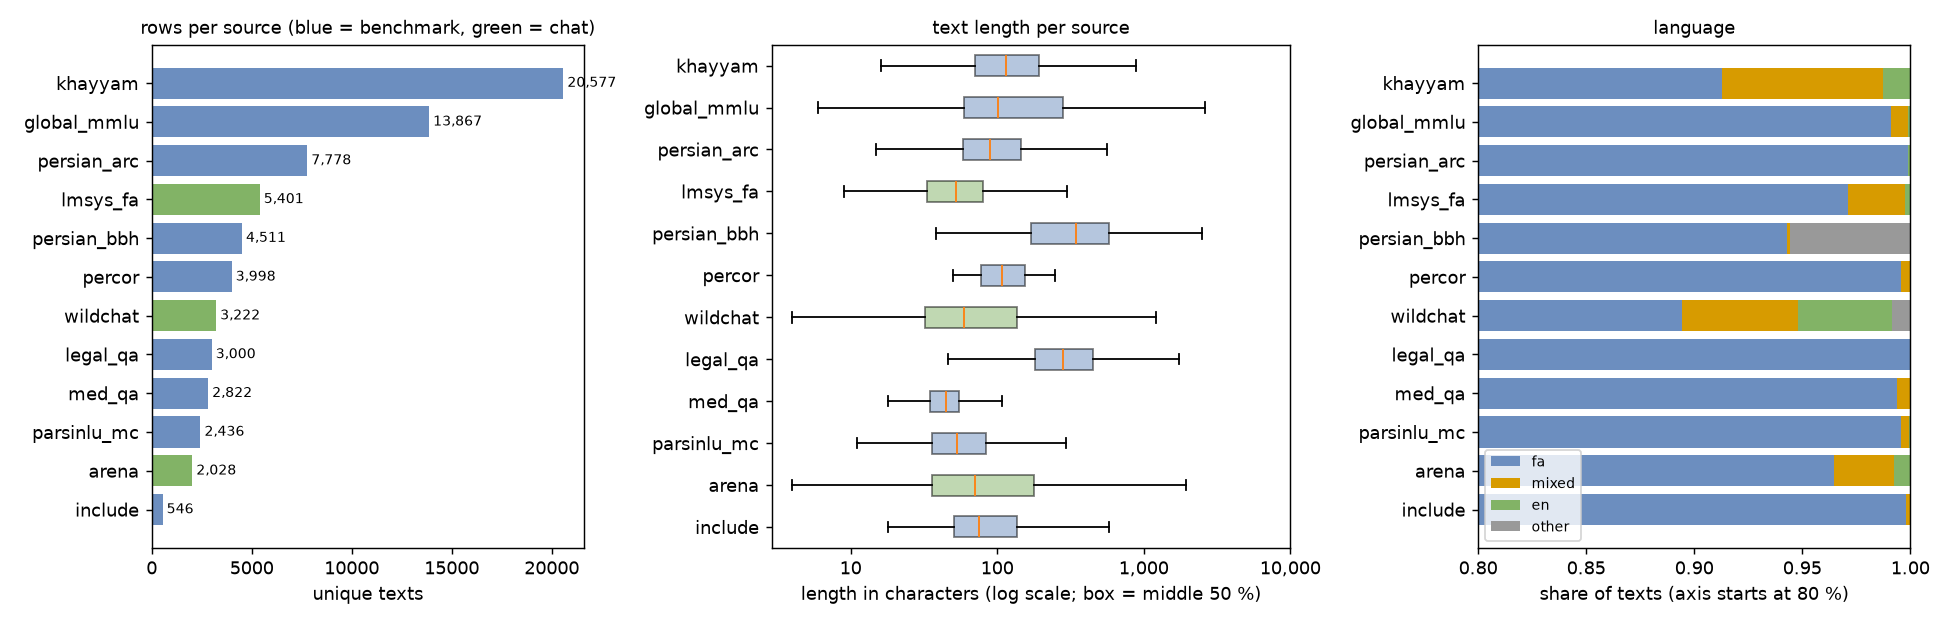
\includegraphics[width=\linewidth]{data_overview.png}
\caption{Data overview. Left: texts per source (blue benchmark, green chat). Middle: length on a log scale
(box = middle 50\,\%). Right: language mix (axis starts at 80\,\%). Khayyam's ``mixed'' share comes from
formulas; WildChat contains the most English.}
\label{fig:data}
\end{figure}

\subsection{Test sets}

From these sources we build five test sets. Each one mirrors a situation from the paper or from our project:

\begin{center}\small
\begin{tabular}{lrp{9.5cm}}
\toprule
Set & Size & Role \\
\midrule
mix & 28{,}802 & nine benchmarks, at most 4{,}000 each; mirrors \textbf{EmbedLLM} (a mix of benchmarks) \\
Khayyam & 20{,}577 & native Persian school exams; 38 categories, 95 courses, 5 difficulty levels, examinee answer rates \\
Global-MMLU & 13{,}867 & machine-translated MMLU; 57 subjects in 6 categories \\
one topic & 1{,}672 & Khayyam's largest category (upper-secondary Persian literature); mirrors \textbf{Headlines} \\
chat & 10{,}651 & lmsys (5{,}401), WildChat (3{,}222), Arena (2{,}028); no labels; closest to Metis traffic \\
\bottomrule
\end{tabular}
\end{center}

%=====================================================================
\section{Method}
%=====================================================================

\begin{figure}[H]
\centering
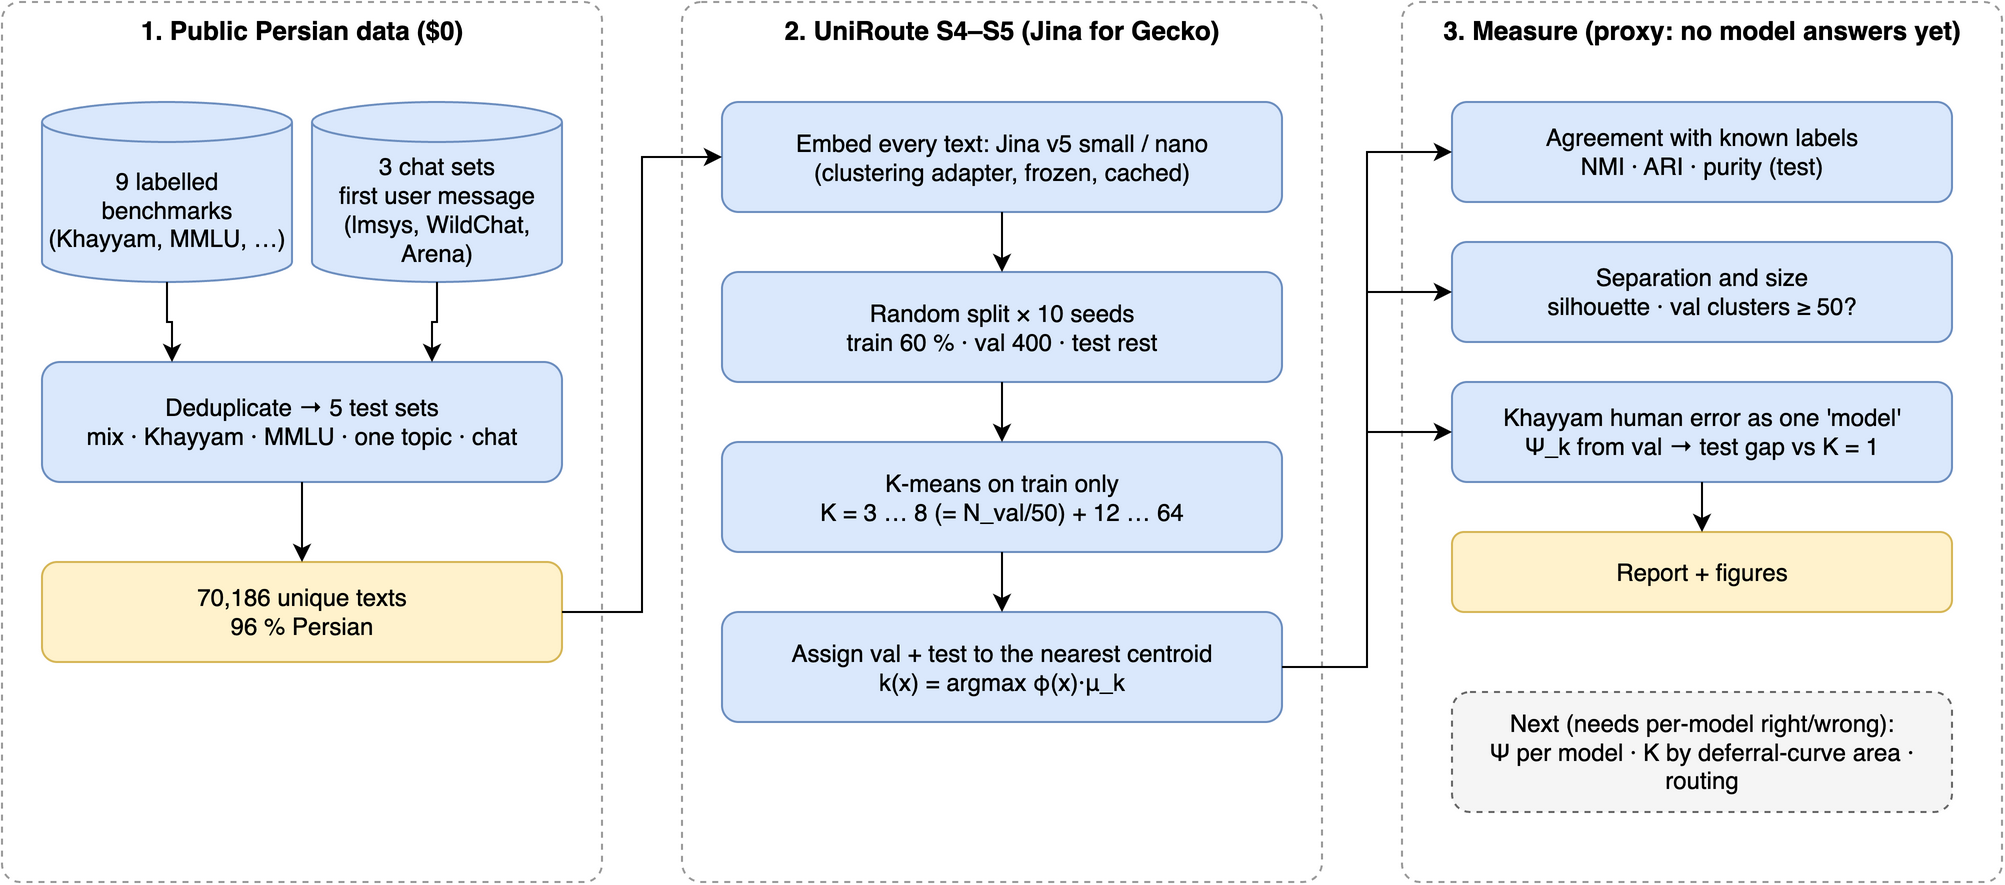
\includegraphics[width=\linewidth]{pipeline.png}
\caption{Pipeline of this study. Blue: free, offline steps; yellow: totals and outputs; grey: what still needs
per-model labels.}
\label{fig:pipeline}
\end{figure}

\subsection{Protocol (as in the paper)}

\begin{itemize}
\item \textbf{Embedding.} Every unique text is embedded once with each embedder and cached by text hash. Inputs
are capped at 2{,}048 tokens for this test; this affects 111 (small) / 71 (nano) chat messages.
\item \textbf{Split.} For each set and each of $R$ random seeds: train = 60\,\%, validation = 400 prompts
(the project's $N_{\mathrm{val}}$), test = the rest. The paper uses 400 repeats; we use $R=10$ for
$K\le8$ and $R=3$ for larger $K$.
\item \textbf{Clustering.} $K$-means (k-means++, 10 restarts, seed recorded) is fitted on the train part only.
Validation and test prompts are assigned with Eq.~\eqref{eq:assign}.
\item \textbf{$K$ grid.} The paper's range $3\dots N_{\mathrm{val}}/50 = 3\dots8$, plus $K\in\{12,16,24,32,48,64\}$
and $K$ = number of known classes, as references.
\item \textbf{Statistics.} We report the mean over splits with a 95\,\% $t$-interval.
\end{itemize}

\subsection{Measures}

The paper chooses $K$ by routing quality, which needs per-model labels. We use measures that do not need them.

\begin{description}
\item[NMI] Normalised mutual information between test clusters and a known label: 0 = unrelated, 1 = identical.
We also report the NMI with shuffled labels as the chance level.
\item[ARI, purity] Adjusted Rand index, and the share of test prompts that carry their cluster's most common label.
\item[Silhouette] Cosine silhouette on up to 3{,}000 test prompts: how much closer a prompt is to its own cluster
than to the next one. It needs no labels.
\item[Cluster size] The number of validation clusters with fewer than 50 prompts. The spec (S5) requires
$|C_k|\ge50$ for every cluster.
\item[Composition] For one split at $K=8$, the label mix of every cluster, and for every label the share of its
prompts that land in its main cluster (``loyalty'').
\item[Topic anchors] For unlabelled chat, we wrote 13 short topic descriptions in Persian and English (e.g.\ programming,
law, poetry, small talk) and embedded them with the same model. Each prompt gets its nearest topic, and we report
the topic mix per cluster. We validate the method on Khayyam, where subjects are known.
\end{description}

\subsection{A routing proxy: human difficulty}\label{sec:proxy}

Khayyam records, for 16{,}777 questions, the share of examinees who chose each option. We treat ``the examinees''
as one model with error $e(x)=1-$(share choosing the key); blank answers count as wrong. In the spirit of
Eq.~\eqref{eq:psi}, $\Psi_k=\overline{e}$ over the validation prompts of cluster $k$. On test prompts we measure the
gap that Proposition~2 relates to routing loss, relative to one average for all prompts ($K=1$):
\begin{equation}
\text{gap shrink}(K)=1-\frac{\mathbb E_{\text{test}}\,|e(x)-\Psi_{k(x)}|}{\mathbb E_{\text{test}}\,|e(x)-\overline e|}.
\end{equation}
We compute $\Psi$ twice. Once from the 400 validation prompts, which is the paper's setting. Once from the large
train part, which is free of sampling noise. The difference between the two isolates the effect of the small
validation set.

\subsection{Environment}
Apple M1 Pro (16\,GB), PyTorch MPS, scikit-learn $K$-means, UMAP for the maps. A full run took 13 (nano) and
21 (small) minutes including new embeddings. Code: \texttt{scripts/s4\_persian\_cluster.py} and companions
(Appendix~\ref{app:repro}).

%=====================================================================
\section{Results}
%=====================================================================

\subsection{Do clusters recover known topics? (RQ1, RQ2)}

\begin{figure}[H]
\centering
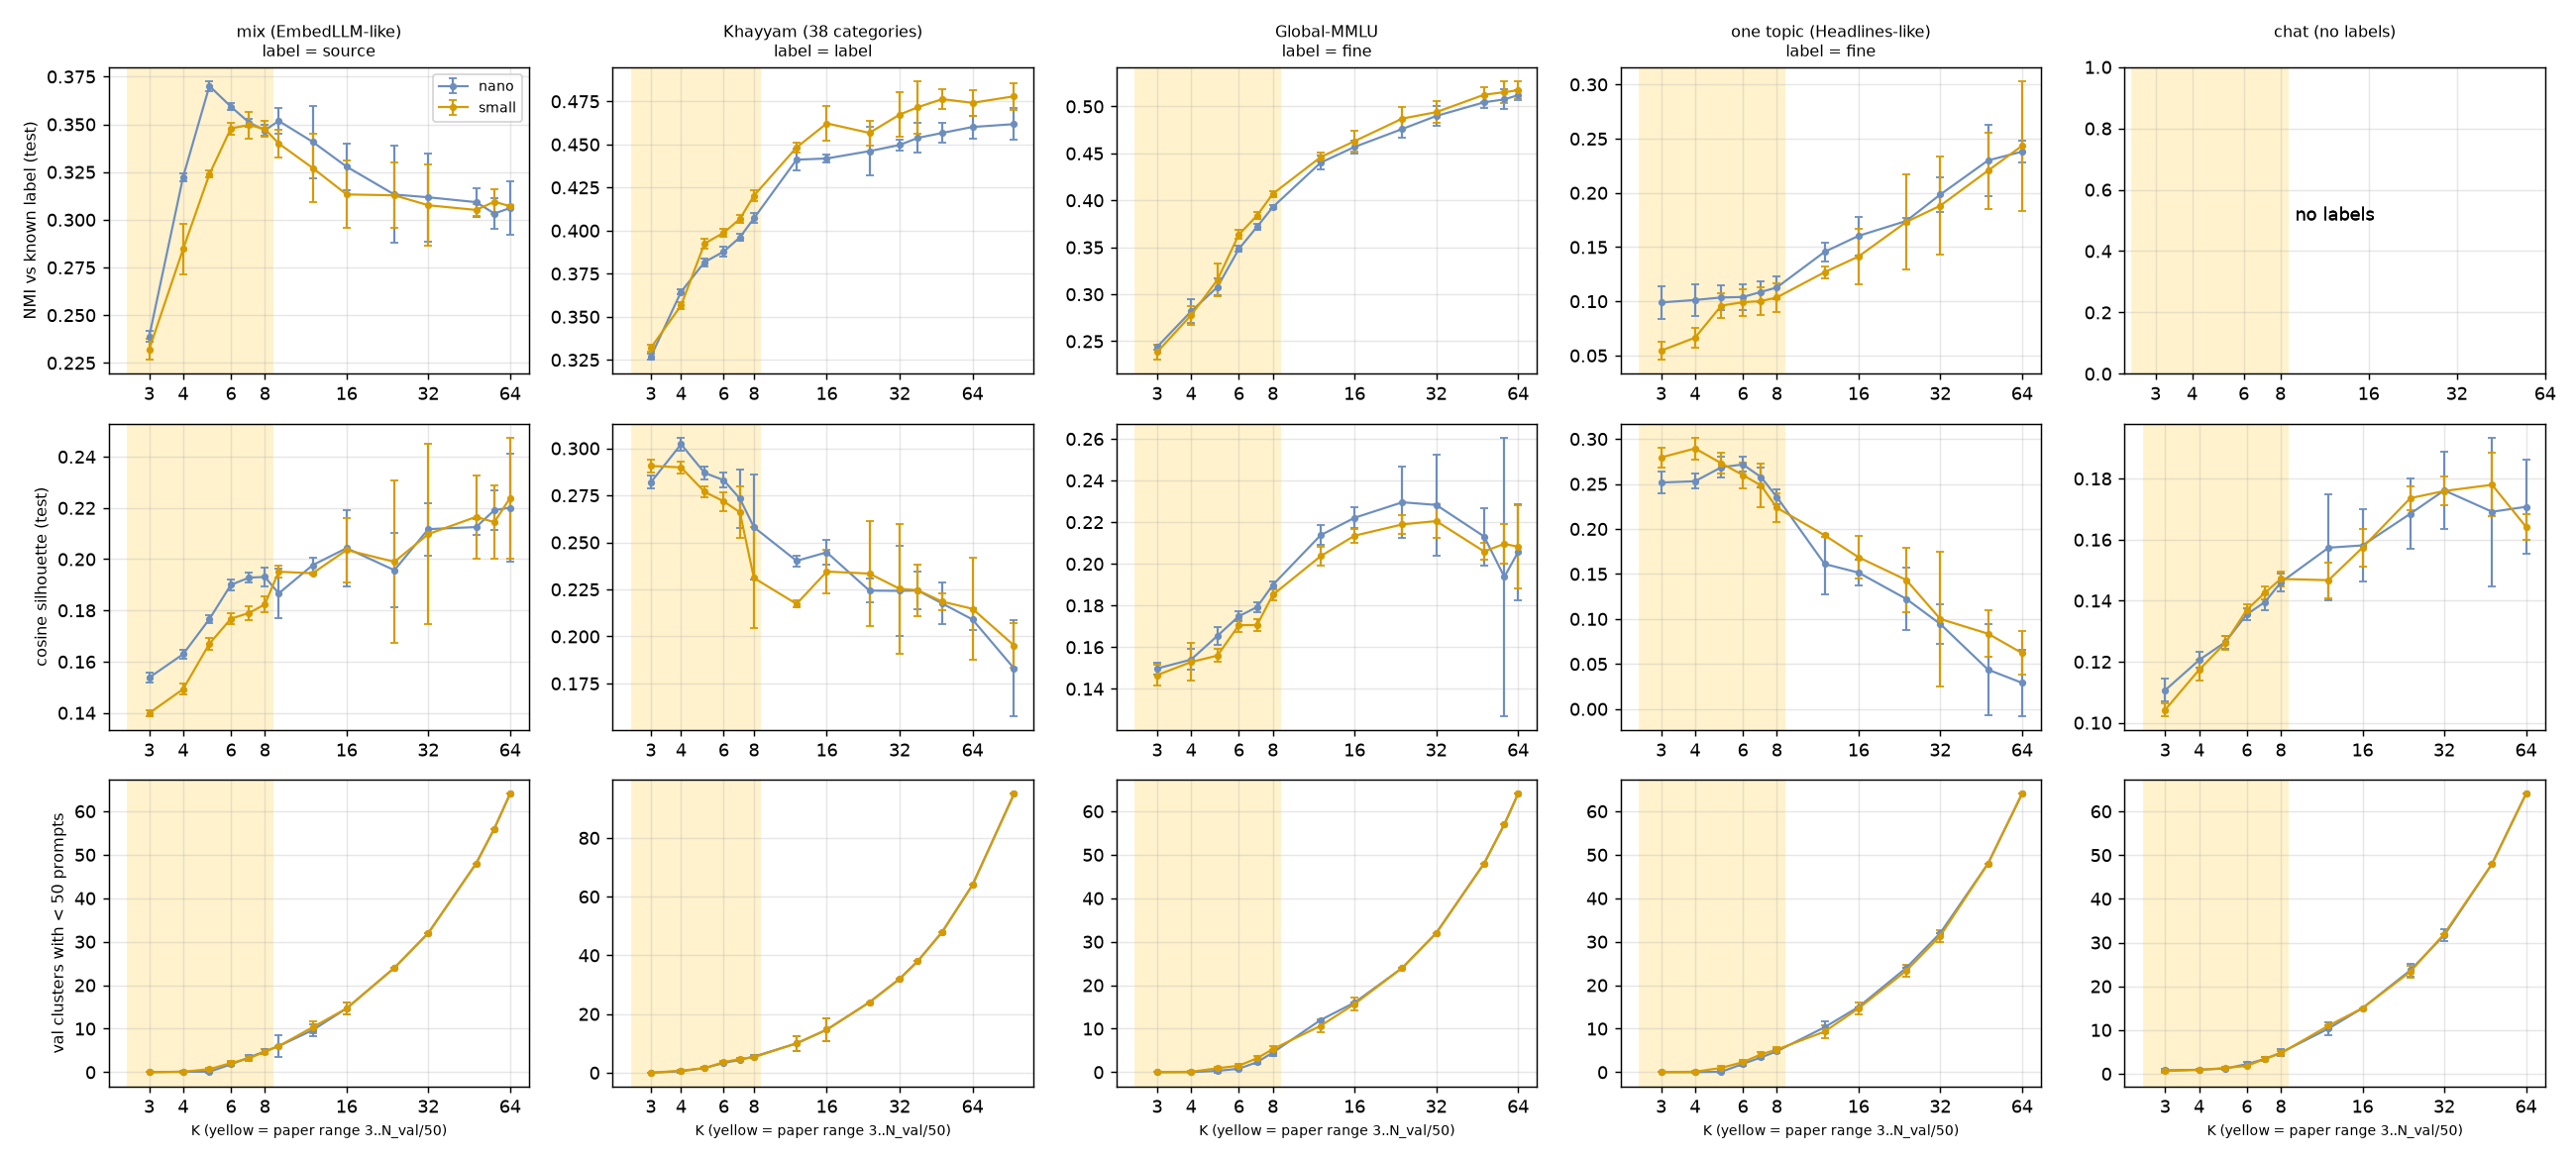
\includegraphics[width=\linewidth]{k_curves.png}
\caption{Scores against $K$ for both embedders (mean and 95\,\% CI over splits). Top: NMI against the known
label. Middle: cosine silhouette. Bottom: validation clusters with fewer than 50 prompts. Yellow band = the
paper's range $K=3\dots8$ for $N_{\mathrm{val}}=400$.}
\label{fig:k}
\end{figure}

\begin{table}[H]
\centering\small
\caption{Paper range $K=3\dots8$: NMI ($\pm$ 95\,\% CI over 10 splits), silhouette, and number of validation
clusters with fewer than 50 prompts. Labels: mix = source, Khayyam = 38 categories, Global-MMLU = 57 subjects,
one topic = 6 courses.}
\label{tab:main}
\begin{tabular}{llrrrrrr}
\toprule
 & & \multicolumn{3}{c}{small} & \multicolumn{3}{c}{nano} \\
\cmidrule(lr){3-5}\cmidrule(lr){6-8}
Set & $K$ & NMI & Sil. & $<50$ & NMI & Sil. & $<50$ \\
\midrule
\multirow{6}{*}{mix} & 3 & 0.232 $\pm$ 0.005 & 0.140 & 0.0 & 0.239 $\pm$ 0.003 & 0.154 & 0.0 \\
 & 4 & 0.285 $\pm$ 0.013 & 0.149 & 0.1 & 0.322 $\pm$ 0.002 & 0.163 & 0.1 \\
 & 5 & 0.324 $\pm$ 0.002 & 0.167 & 0.7 & 0.370 $\pm$ 0.003 & 0.177 & 0.1 \\
 & 6 & 0.348 $\pm$ 0.003 & 0.177 & 2.1 & 0.359 $\pm$ 0.002 & 0.190 & 1.8 \\
 & 7 & 0.350 $\pm$ 0.007 & 0.179 & 3.2 & 0.351 $\pm$ 0.002 & 0.193 & 3.4 \\
 & 8 & 0.348 $\pm$ 0.004 & 0.182 & 4.7 & 0.347 $\pm$ 0.003 & 0.193 & 4.8 \\
\midrule
\multirow{6}{*}{Khayyam} & 3 & 0.332 $\pm$ 0.002 & 0.291 & 0.0 & 0.327 $\pm$ 0.002 & 0.282 & 0.0 \\
 & 4 & 0.357 $\pm$ 0.002 & 0.290 & 0.7 & 0.364 $\pm$ 0.002 & 0.302 & 0.5 \\
 & 5 & 0.392 $\pm$ 0.003 & 0.277 & 1.6 & 0.382 $\pm$ 0.002 & 0.287 & 1.6 \\
 & 6 & 0.399 $\pm$ 0.002 & 0.272 & 3.6 & 0.388 $\pm$ 0.003 & 0.283 & 3.3 \\
 & 7 & 0.407 $\pm$ 0.002 & 0.266 & 4.7 & 0.396 $\pm$ 0.002 & 0.273 & 4.4 \\
 & 8 & 0.420 $\pm$ 0.003 & 0.231 & 5.3 & 0.407 $\pm$ 0.003 & 0.258 & 5.5 \\
\midrule
\multirow{6}{*}{Global-MMLU} & 3 & 0.238 $\pm$ 0.008 & 0.147 & 0.0 & 0.244 $\pm$ 0.003 & 0.150 & 0.0 \\
 & 4 & 0.278 $\pm$ 0.010 & 0.153 & 0.1 & 0.282 $\pm$ 0.013 & 0.154 & 0.0 \\
 & 5 & 0.315 $\pm$ 0.017 & 0.156 & 0.9 & 0.308 $\pm$ 0.009 & 0.165 & 0.3 \\
 & 6 & 0.364 $\pm$ 0.005 & 0.171 & 1.5 & 0.348 $\pm$ 0.003 & 0.175 & 0.8 \\
 & 7 & 0.384 $\pm$ 0.004 & 0.171 & 3.2 & 0.372 $\pm$ 0.003 & 0.179 & 2.3 \\
 & 8 & 0.407 $\pm$ 0.003 & 0.185 & 5.3 & 0.393 $\pm$ 0.002 & 0.190 & 4.5 \\
\midrule
\multirow{6}{*}{one topic} & 3 & 0.054 $\pm$ 0.008 & 0.279 & 0.0 & 0.099 $\pm$ 0.015 & 0.252 & 0.0 \\
 & 4 & 0.066 $\pm$ 0.009 & 0.289 & 0.1 & 0.101 $\pm$ 0.015 & 0.253 & 0.0 \\
 & 5 & 0.096 $\pm$ 0.012 & 0.273 & 1.0 & 0.104 $\pm$ 0.011 & 0.269 & 0.1 \\
 & 6 & 0.099 $\pm$ 0.012 & 0.260 & 2.3 & 0.104 $\pm$ 0.012 & 0.272 & 1.9 \\
 & 7 & 0.100 $\pm$ 0.013 & 0.248 & 4.1 & 0.109 $\pm$ 0.010 & 0.258 & 3.4 \\
 & 8 & 0.104 $\pm$ 0.013 & 0.224 & 5.2 & 0.113 $\pm$ 0.011 & 0.236 & 4.8 \\
\midrule
\multirow{6}{*}{chat} & 3 & -- & 0.104 & 0.6 & -- & 0.111 & 0.8 \\
 & 4 & -- & 0.117 & 0.9 & -- & 0.121 & 0.9 \\
 & 5 & -- & 0.126 & 1.3 & -- & 0.126 & 1.2 \\
 & 6 & -- & 0.137 & 1.8 & -- & 0.136 & 2.2 \\
 & 7 & -- & 0.143 & 3.4 & -- & 0.140 & 3.4 \\
 & 8 & -- & 0.147 & 4.7 & -- & 0.146 & 4.8 \\
\bottomrule
\end{tabular}

\end{table}

\begin{itemize}
\item \textbf{Benchmark mix.} NMI against the nine sources rises from 0.23 ($K=3$) to 0.35--0.37 at $K=5$--8, then
falls slightly. Most sources form their own clusters (\S\ref{sec:meaning}).
\item \textbf{Subject-rich sets.} On Khayyam (38 categories) and Global-MMLU (57 subjects), NMI keeps rising with $K$
(Khayyam 0.33 $\to$ 0.42 at $K=8$ $\to$ 0.47 at $K=38$; MMLU 0.24 $\to$ 0.41 $\to$ 0.52 at $K=64$). These sets have
more real subjects than eight clusters can hold.
\item \textbf{One topic.} NMI stays near 0.10 in the paper range, and the silhouette falls quickly with $K$:
there is little structure to find. This reproduces the paper's EmbedLLM-versus-Headlines contrast (\textbf{RQ2}).
\item \textbf{Chat.} Silhouette 0.10--0.15 in the paper range, against 0.15--0.30 for the benchmarks.
Chat clusters exist but are softer.
\item \textbf{Cluster sizes.} With 400 validation prompts, $K=8$ leaves on average about five of eight validation
clusters below 50 prompts. Already at $K=5$, one cluster often falls below 50.
\end{itemize}

\subsection{small vs.\ nano vs.\ adapters (RQ3)}

\begin{figure}[H]
\centering
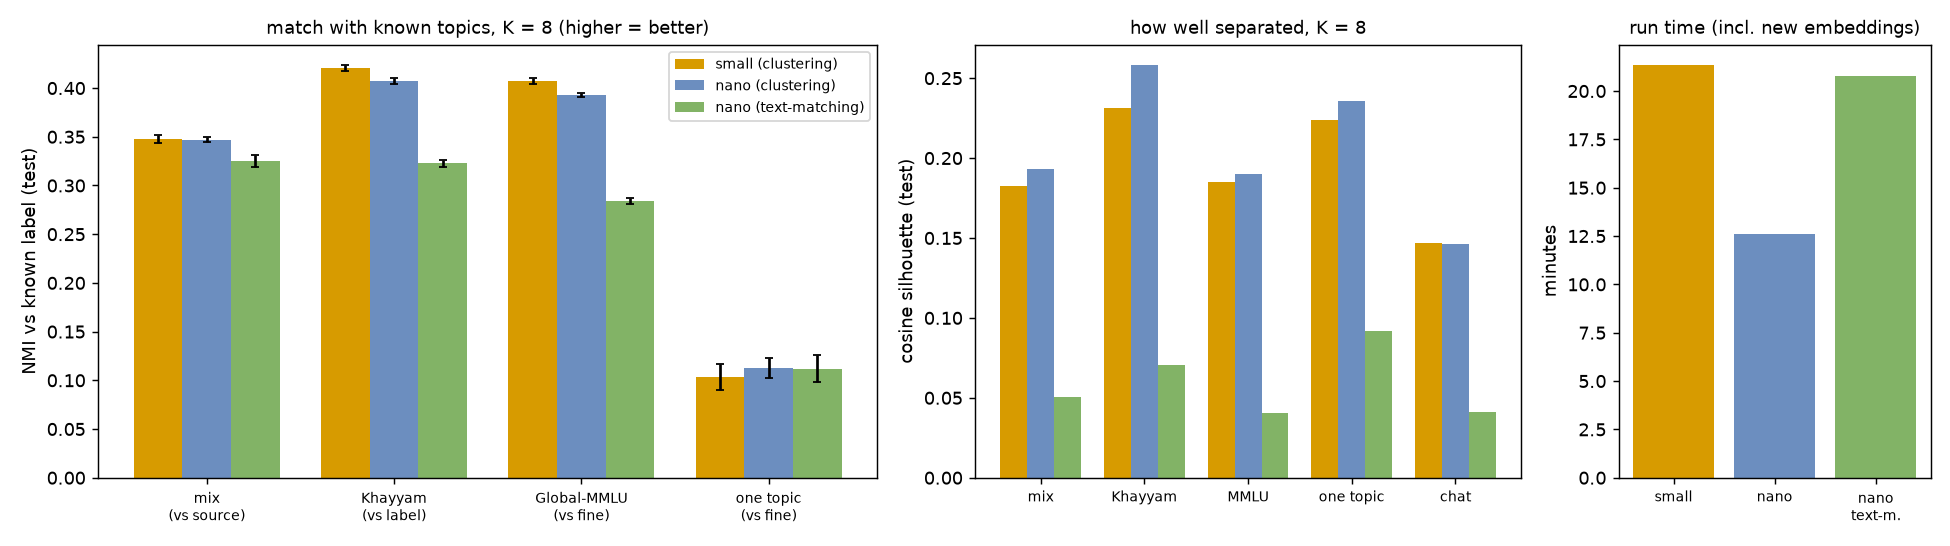
\includegraphics[width=\linewidth]{model_compare.png}
\caption{At $K=8$: NMI against known labels, silhouette, and run time for small, nano and nano with the
\texttt{text-matching} adapter.}
\label{fig:compare}
\end{figure}

\begin{table}[H]
\centering\small
\caption{Embedder comparison at $K=8$ (NMI $\pm$ 95\,\% CI; chat: silhouette).}
\label{tab:compare}
\begin{tabular}{lccc}
\toprule
$K = 8$ & small & nano & nano (text-m.) \\
\midrule
mix (source) & 0.348 $\pm$ 0.004 & 0.347 $\pm$ 0.003 & 0.325 $\pm$ 0.006 \\
Khayyam (label) & 0.420 $\pm$ 0.003 & 0.407 $\pm$ 0.003 & 0.323 $\pm$ 0.004 \\
Global-MMLU (fine) & 0.407 $\pm$ 0.003 & 0.393 $\pm$ 0.002 & 0.284 $\pm$ 0.003 \\
one topic (fine) & 0.104 $\pm$ 0.013 & 0.113 $\pm$ 0.011 & 0.112 $\pm$ 0.014 \\
chat (no labels) & sil. 0.147 & sil. 0.146 & sil. 0.041 \\
Khayyam difficulty gap shrink & 5.4\% $\pm$ 0.6\% & 5.4\% $\pm$ 0.4\% & 7.7\% $\pm$ 0.5\% \\
Run time (min) & 21 & 13 & 21 \\
\bottomrule
\end{tabular}

\end{table}

\emph{small} beats \emph{nano} by 0.013--0.014 NMI on the two subject-rich sets. \emph{nano} wins on the mix at
$K=4$--5 (0.370 vs.\ 0.324 at $K=5$) and on the single topic, and it is better separated on every labelled set.
Both shrink the Khayyam difficulty gap equally. For clustering alone, the two are interchangeable, and nano is
faster and the only one that meets the latency budget. The \texttt{text-matching} adapter clusters clearly worse:
NMI 0.08--0.12 lower, silhouette near 0.05, and lopsided cluster sizes. Unexpectedly, its difficulty gain is larger
(7.7\,\%); we return to this in \S\ref{sec:discussion}.

\subsection{Cluster maps}

Figure~\ref{fig:maps} projects 6{,}000 test prompts per set to two dimensions with UMAP. On the left, dots are
coloured by $K$-means cluster ($K=8$); on the right, by known label. Where the coloured islands on both sides
coincide, the clusters follow the labels.

\begin{figure}[H]
\centering
\begin{subfigure}{\linewidth}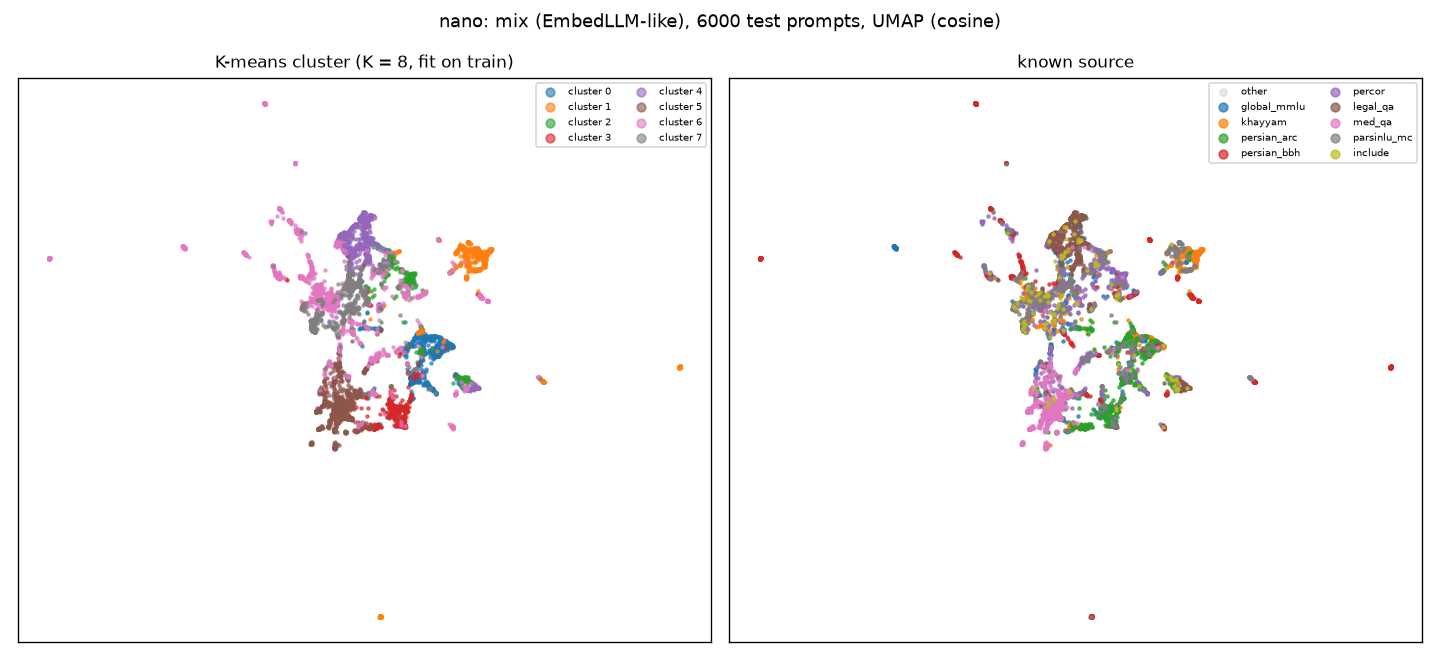
\includegraphics[width=\linewidth]{map_nano_mix.png}\caption{mix: right = source}\end{subfigure}
\begin{subfigure}{\linewidth}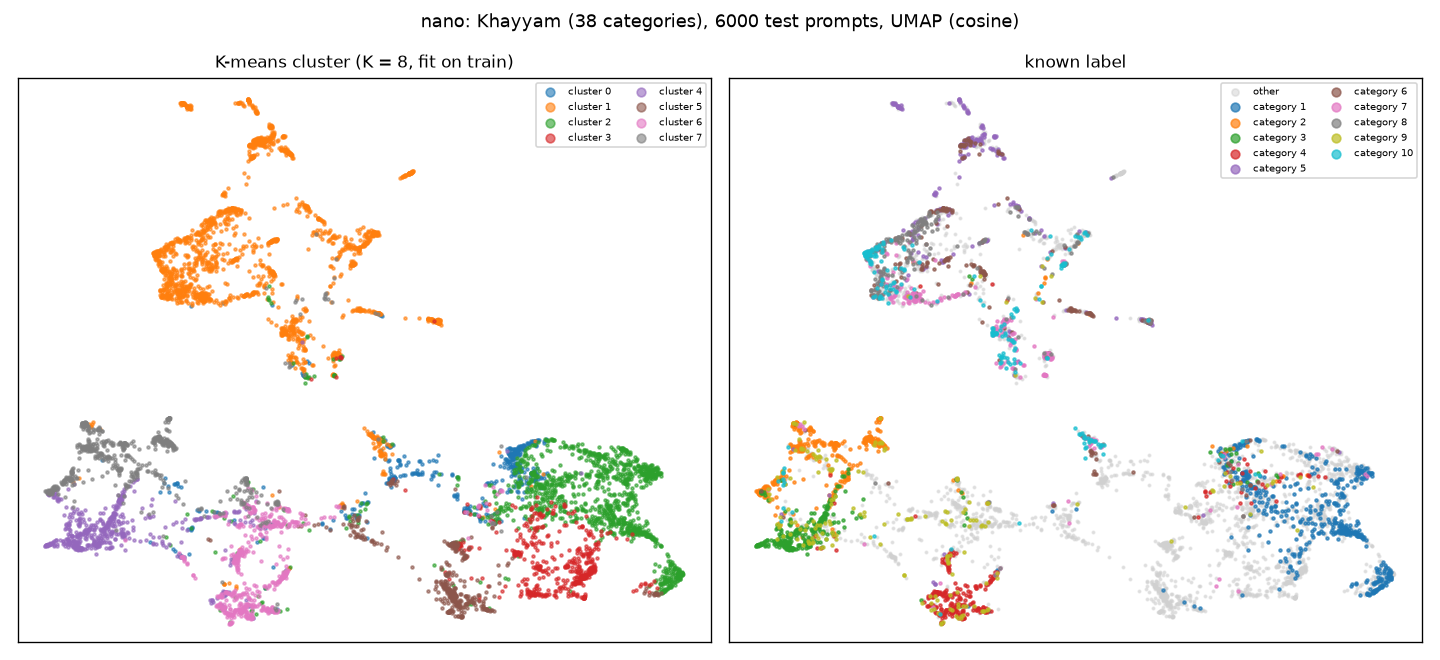
\includegraphics[width=\linewidth]{map_nano_khayyam.png}\caption{Khayyam: right = ten largest categories (numbered as in Fig.~\ref{fig:compkh})}\end{subfigure}
\caption{UMAP maps (nano, $K=8$, one split, test prompts).}
\label{fig:maps}
\end{figure}
\begin{figure}[H]
\ContinuedFloat
\centering
\begin{subfigure}{\linewidth}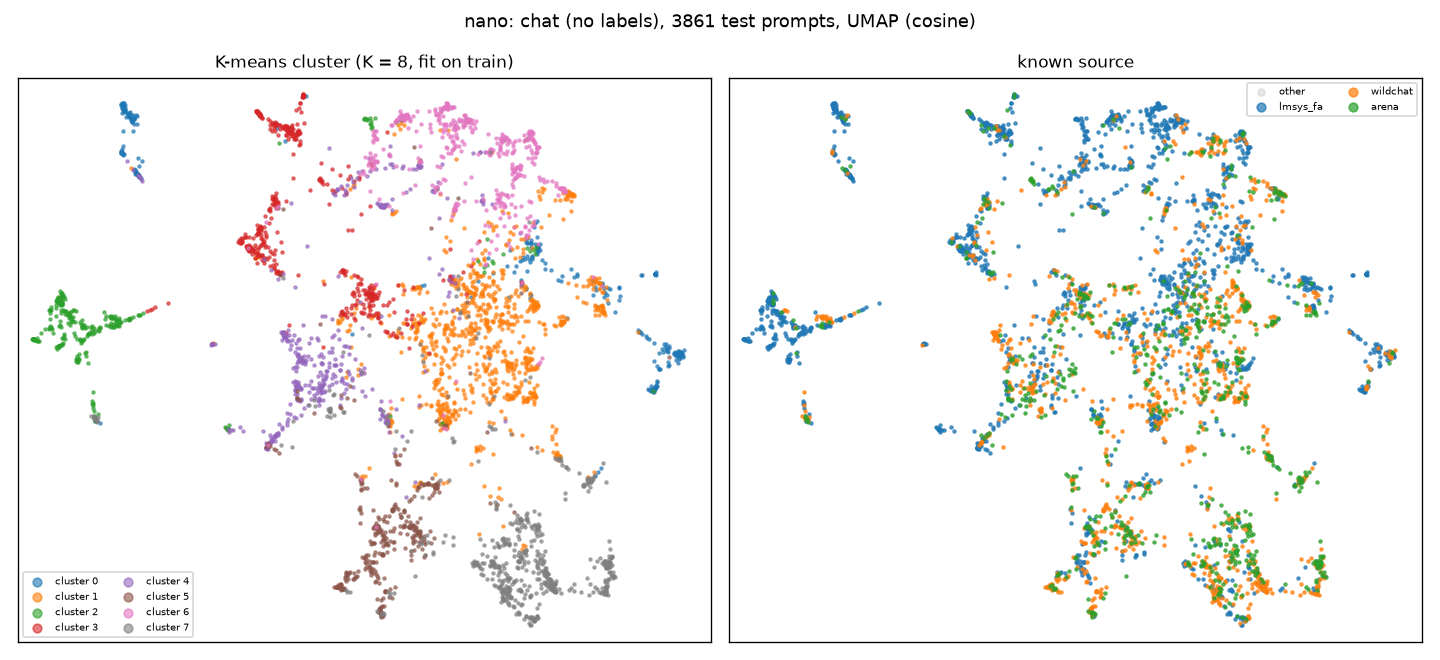
\includegraphics[width=\linewidth]{map_nano_chat.png}\caption{chat: right = source dataset}\end{subfigure}
\caption{(continued) On chat, the three sources are largely mixed; clusters follow what is asked, not where the data came from.}
\end{figure}

\subsection{Are the clusters meaningful? (RQ4)}\label{sec:meaning}

\paragraph{Better than chance.} At $K=8$ (nano, one split), NMI against the known label is far above the shuffled
baseline: Khayyam 0.405 vs.\ 0.005, Global-MMLU subjects 0.392 vs.\ 0.015, mix sources 0.350 vs.\ 0.001. Khayyam's
difficulty \emph{level} reaches only 0.009, so clusters group by subject, not by difficulty.

\paragraph{Benchmark mix.}

\begin{figure}[H]
\centering
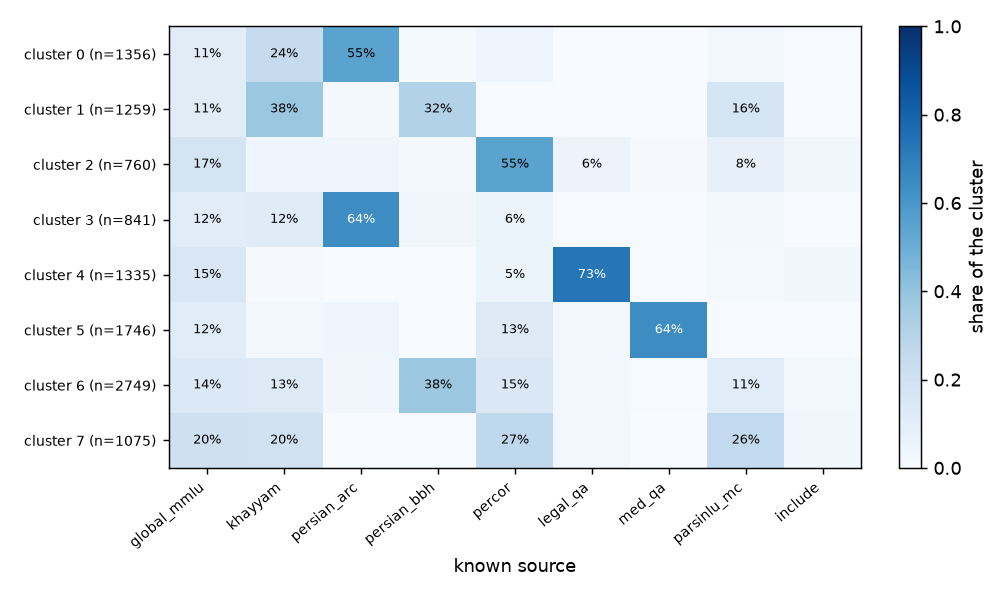
\includegraphics[width=.85\linewidth]{composition_mix.png}
\caption{mix: share of each source inside each cluster (rows sum to 100\,\%).}
\label{fig:compmix}
\end{figure}

\begin{table}[H]
\centering\small
\caption{mix: largest sources per cluster.}
\begin{tabular}{rr>{\raggedright\arraybackslash}p{10cm}}
\toprule
\# & $n$ & Largest sources (share of cluster) \\
\midrule
0 & 1,356 & \footnotesize persian\_arc 55\%; khayyam 24\%; global\_mmlu 11\%; percor 5\% \\
1 & 1,259 & \footnotesize khayyam 38\%; persian\_bbh 32\%; parsinlu\_mc 16\%; global\_mmlu 11\% \\
2 & 760 & \footnotesize percor 55\%; global\_mmlu 17\%; parsinlu\_mc 8\%; legal\_qa 6\% \\
3 & 841 & \footnotesize persian\_arc 64\%; khayyam 12\%; global\_mmlu 12\%; percor 6\% \\
4 & 1,335 & \footnotesize legal\_qa 73\%; global\_mmlu 15\%; percor 5\%; include 3\% \\
5 & 1,746 & \footnotesize med\_qa 64\%; percor 13\%; global\_mmlu 12\%; persian\_arc 5\% \\
6 & 2,749 & \footnotesize persian\_bbh 38\%; percor 15\%; global\_mmlu 14\%; khayyam 13\% \\
7 & 1,075 & \footnotesize percor 27\%; parsinlu\_mc 26\%; global\_mmlu 20\%; khayyam 20\% \\
\bottomrule
\end{tabular}

\end{table}

Legal QA (73\,\% of cluster 4), medical QA (64\,\% of cluster 5), PerCoR news and commonsense (55\,\% of cluster 2)
and Persian ARC science (clusters 0 and 3) each dominate a cluster. Reasoning puzzles from BBH share clusters 1 and 6
with Khayyam's mathematics and logic questions. Clusters follow \emph{what is asked}, not \emph{which dataset} the
question came from. Global-MMLU spreads over all clusters because it covers 57 subjects.

\paragraph{Khayyam.}

\begin{figure}[H]
\centering
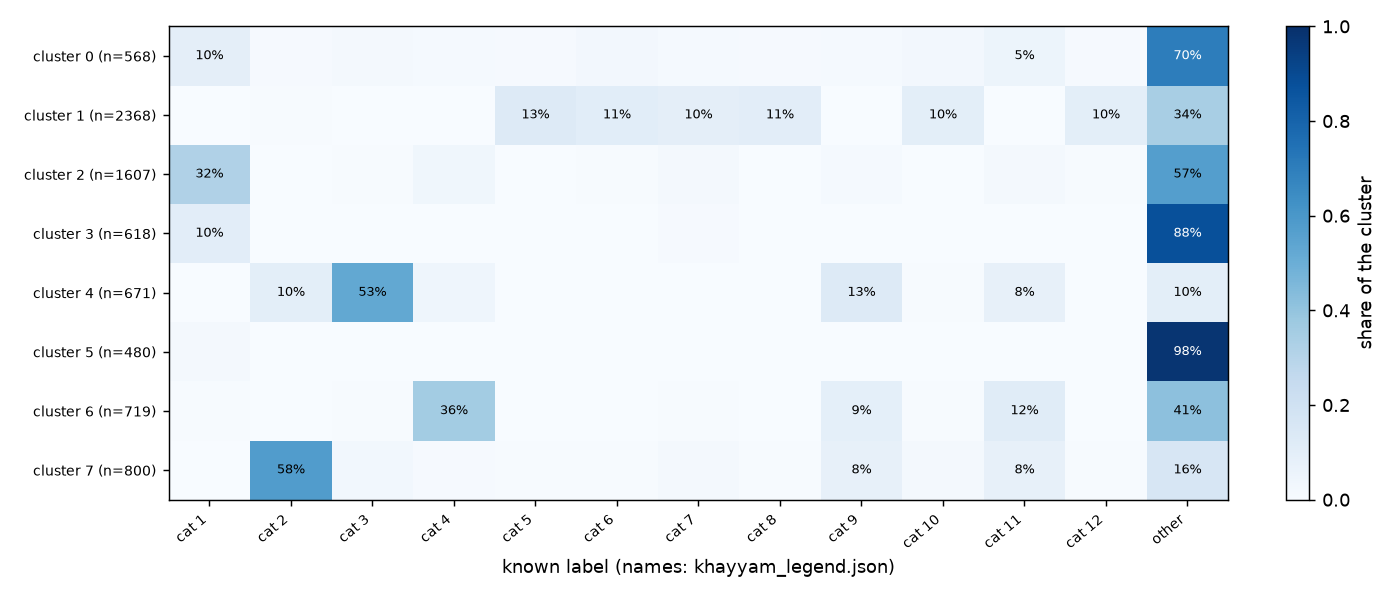
\includegraphics[width=\linewidth]{composition_khayyam.png}
\caption{Khayyam: share of the twelve largest categories inside each cluster. cat~1 Persian literature (upper sec.),
2 physics, 3 chemistry, 4 biology, 5 mathematics (upper sec.), 6 mathematics \& statistics, 7 mathematical \& logical IQ
(upper prim.), 8 mathematics (lower sec.), 9 science (lower sec.), 10 mathematics (upper prim.), 11 science (upper prim.),
12 geometry; ``other'' = the 26 smaller categories.}
\label{fig:compkh}
\end{figure}

\begin{table}[H]
\centering\small
\caption{Khayyam clusters ($K=8$, nano, test prompts): name, size, largest categories, and mean examinee error.}
\label{tab:khcl}
\begin{tabular}{rlr>{\raggedright\arraybackslash}p{8.2cm}r}
\toprule
\# & Name & $n$ & Largest categories (share of cluster) & Error \\
\midrule
0 & humanities mix & 568 & \footnotesize Psychology (upper sec.) 11\%; Economics (upper sec.) 10\%; Persian literature (upper sec.) 10\% & 0.54 \\
1 & mathematics & 2,368 & \footnotesize Mathematics (upper sec.) 13\%; Calculus (upper sec.) 12\%; Mathematics \& statistics (upper sec.) 11\% & 0.71 \\
2 & Persian literature & 1,607 & \footnotesize Persian literature (upper sec.) 32\%; Persian literature (lower sec.) 10\%; Persian literature (upper prim.) 10\% & 0.56 \\
3 & religion \& philosophy & 618 & \footnotesize Philosophy (upper sec.) 18\%; Islamic education (upper prim.) 11\%; Persian literature (upper sec.) 10\% & 0.56 \\
4 & chemistry & 671 & \footnotesize Chemistry (upper sec.) 53\%; Science (lower sec.) 13\%; Physics (upper sec.) 10\% & 0.66 \\
5 & history \& society & 480 & \footnotesize History (upper sec.) 38\%; Sociology (upper sec.) 20\%; Social studies (lower sec.) 14\% & 0.58 \\
6 & biology \& science & 719 & \footnotesize Biology (upper sec.) 36\%; Science (upper prim.) 12\%; Geography (upper sec.) 10\% & 0.57 \\
7 & physics & 800 & \footnotesize Physics (upper sec.) 58\%; Science (lower sec.) 8\%; Science (upper prim.) 8\% & 0.69 \\
\bottomrule
\end{tabular}

\end{table}

Eight clusters must hold 38 categories, so related subjects share. Every cluster can still be named
(Table~\ref{tab:khcl}), and loyalty is high (Appendix~\ref{app:loyalty}): calculus 99.6\,\%, upper-secondary
mathematics 95\,\%, discrete mathematics 95\,\%, chemistry 87\,\%, physics 83\,\%, Persian literature 79--87\,\% at
all four school levels, religion 83--100\,\%. The errors are sensible. All mathematics merges into one cluster
regardless of grade. Lower-grade ``general science'' and social studies split (30--37\,\% in their main cluster),
which matches their mixed content. Clusters also \textbf{differ in difficulty}: examinees miss 71\,\% of
mathematics and 69\,\% of physics questions, but only 54--58\,\% in the humanities clusters. That is the kind of
signal Eq.~\eqref{eq:route} uses.

\paragraph{Global-MMLU.}

\begin{table}[H]
\centering\small
\caption{Global-MMLU clusters ($K=8$, nano).}
\begin{tabular}{rr>{\raggedright\arraybackslash}p{7.2cm}>{\raggedright\arraybackslash}p{4.2cm}}
\toprule
\# & $n$ & Largest subjects & Largest categories \\
\midrule
0 & 684 & \footnotesize high school macroeconomics 19\%; professional accounting 16\%; high school microeconomics 12\% & \footnotesize Social Sciences 47\%; Business 30\% \\
1 & 542 & \footnotesize conceptual physics 13\%; high school chemistry 12\%; miscellaneous 9\% & \footnotesize STEM 72\%; Other 9\% \\
2 & 806 & \footnotesize professional medicine 12\%; nutrition 12\%; clinical knowledge 10\% & \footnotesize Medical 51\%; STEM 23\% \\
3 & 573 & \footnotesize high school world history 13\%; high school us history 13\%; prehistory 9\% & \footnotesize Humanities 60\%; Social Sciences 28\% \\
4 & 545 & \footnotesize elementary mathematics 21\%; high school mathematics 15\%; high school statistics 7\% & \footnotesize STEM 78\%; Social Sciences 12\% \\
5 & 556 & \footnotesize professional law 85\%; international law 4\%; high school government and politics 3\% & \footnotesize Humanities 92\%; Social Sciences 6\% \\
6 & 639 & \footnotesize professional psychology 13\%; high school psychology 13\%; miscellaneous 8\% & \footnotesize Social Sciences 42\%; Humanities 26\% \\
7 & 802 & \footnotesize moral scenarios 42\%; philosophy 8\%; miscellaneous 7\% & \footnotesize Humanities 71\%; Social Sciences 17\% \\
\bottomrule
\end{tabular}

\end{table}

Each cluster has a clear theme: economics and accounting, physical sciences, medicine, history, mathematics, law
(85\,\% professional law), psychology and philosophy, and moral scenarios. Medical and business questions each land
77\,\% in one cluster. The ``humanities'' category splits into history, law and ethics, which really are different
subjects.

\paragraph{Chat (no labels).} The topic-anchor method agrees with Khayyam's known subject on 71.9\,\% of
6{,}574 mapped questions, against 18.7\,\% by chance. It is rough but informative. Figure~\ref{fig:topics} and
Table~\ref{tab:chat} apply it to chat.

\begin{figure}[H]
\centering
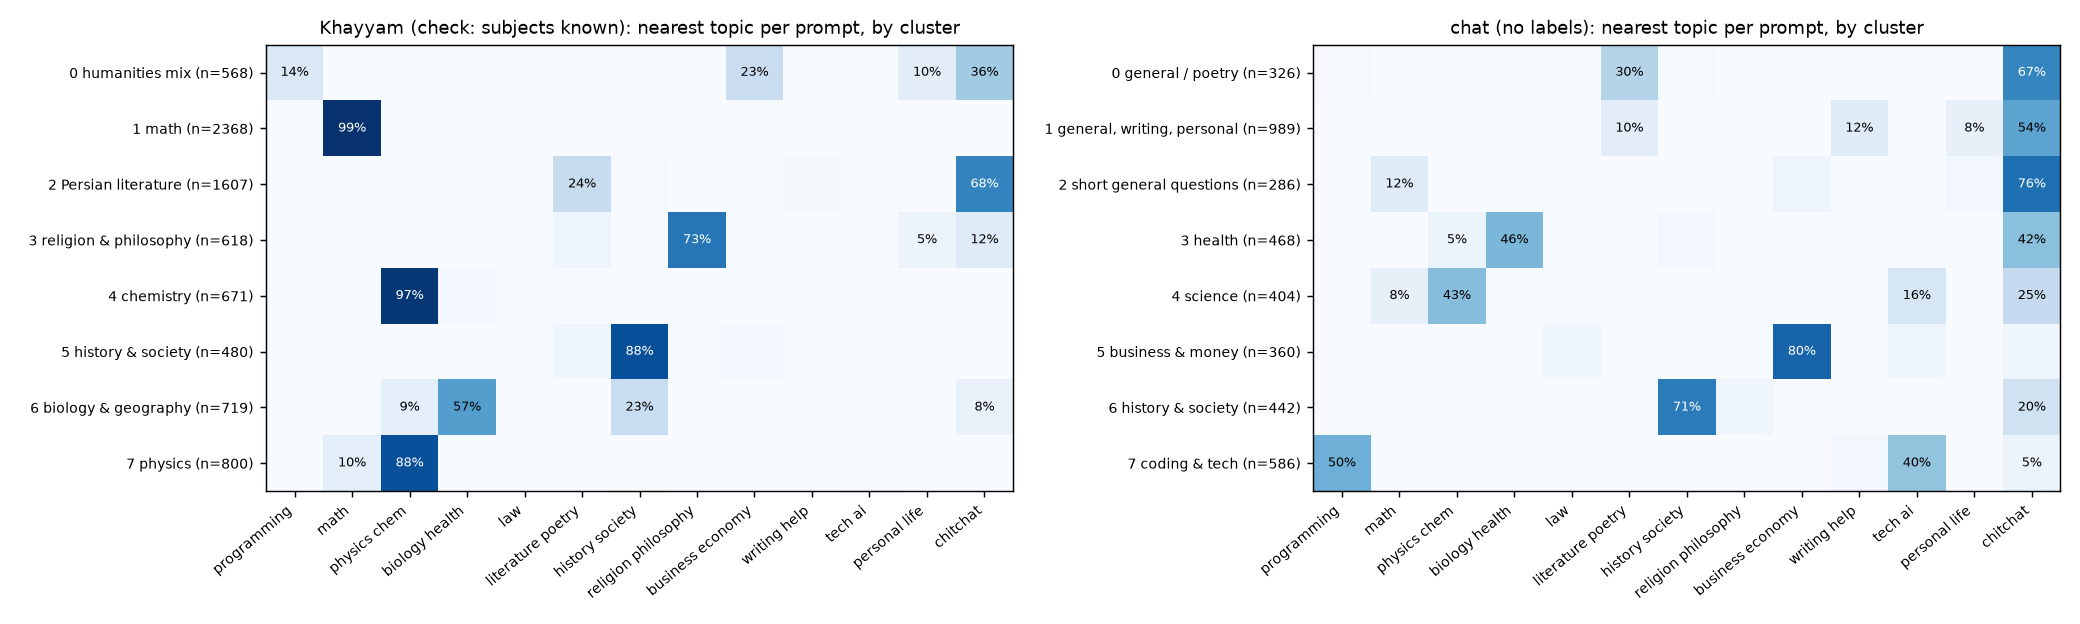
\includegraphics[width=\linewidth]{cluster_topics.png}
\caption{Nearest topic per prompt, by cluster (top four topics per cluster shown). Left: Khayyam, where subjects
are known (validation of the method). Right: chat.}
\label{fig:topics}
\end{figure}

\begin{table}[H]
\centering\small
\caption{Chat clusters ($K=8$, nano). Nearest topic (top three); median length; share of Latin letters; share
with code or math markers; largest source.}
\label{tab:chat}
\resizebox{\linewidth}{!}{\begin{tabular}{rlr>{\raggedright\arraybackslash}p{5.0cm}rrrl}
\toprule
\# & Name & $n$ & Nearest topic & Chars & Latin & Code/math & Main source \\
\midrule
0 & general / poetry & 326 & \footnotesize chitchat 67\%; literature poetry 30\%; history society 2\% & 58 & 3\% & 0\% & lmsys\_fa 82\% \\
1 & general, writing, personal & 989 & \footnotesize chitchat 54\%; writing help 12\%; literature poetry 10\% & 48 & 4\% & 1\% & wildchat 40\% \\
2 & short general questions & 286 & \footnotesize chitchat 76\%; math 12\%; business economy 5\% & 55 & 1\% & 1\% & lmsys\_fa 84\% \\
3 & health & 468 & \footnotesize biology health 46\%; chitchat 42\%; physics chem 5\% & 52 & 2\% & 1\% & lmsys\_fa 69\% \\
4 & science & 404 & \footnotesize physics chem 43\%; chitchat 25\%; tech ai 16\% & 62 & 3\% & 2\% & lmsys\_fa 55\% \\
5 & business \& money & 360 & \footnotesize business economy 80\%; tech ai 4\%; chitchat 4\% & 64 & 5\% & 5\% & wildchat 47\% \\
6 & history \& society & 442 & \footnotesize history society 71\%; chitchat 20\%; religion philosophy 4\% & 50 & 2\% & 1\% & lmsys\_fa 76\% \\
7 & coding \& tech & 586 & \footnotesize programming 50\%; tech ai 40\%; chitchat 5\% & 72 & 10\% & 6\% & wildchat 44\% \\
\bottomrule
\end{tabular}
}
\end{table}

Five of eight chat clusters carry a clear topic. Coding and technology (cluster 7) is also the cluster with the
most Latin script and code markers, which independently confirms the label. The others are business (80\,\%),
history and society (71\,\%), health and science. The remaining three are general, which here also means ``no
anchor fits''. Clusters 0, 2 and 6 come mostly from lmsys\_fa, a translated set, so part of their grouping may
reflect translation style.

\subsection{Would these clusters help routing? (RQ5)}

\begin{figure}[H]
\centering
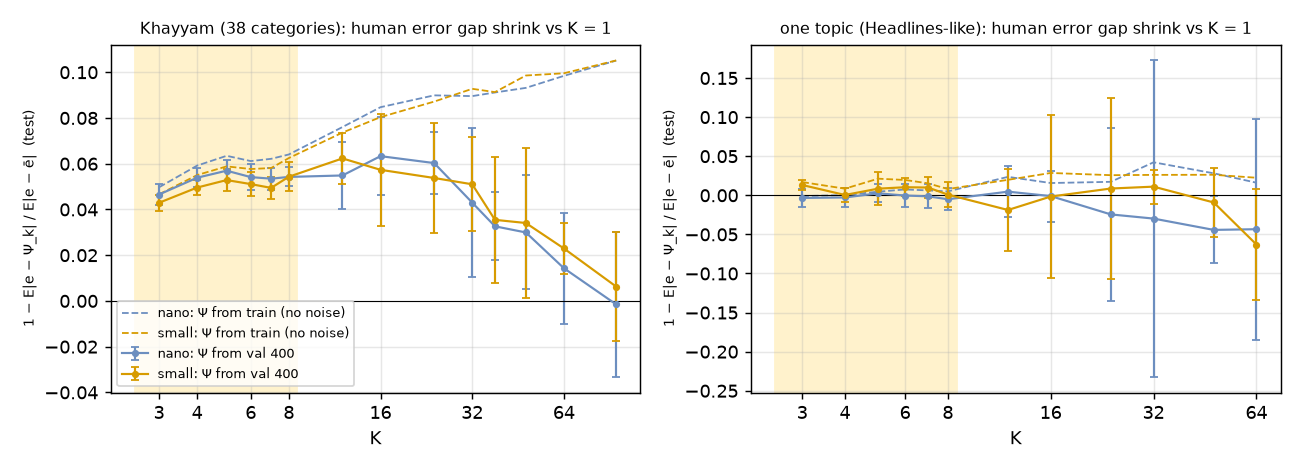
\includegraphics[width=\linewidth]{difficulty_gap.png}
\caption{Gap shrink against $K=1$ on test prompts. Solid: $\Psi$ from 400 validation prompts (paper setting);
dashed: $\Psi$ from the large train part.}
\label{fig:diff}
\end{figure}

\begin{table}[H]
\centering\small
\caption{Gap shrink in \% (validation rows: $\pm$ 95\,\% CI).}
\label{tab:diff}
\begin{tabular}{lllrrrrrr}
\toprule
Set & Model & Profile & $K=3$ & $K=5$ & $K=8$ & $K=16$ & $K=32$ & $K=64$ \\
\midrule
Khayyam & small & $\Psi$ from val (400) & 4.3$\pm$0.3 & 5.3$\pm$0.5 & 5.4$\pm$0.6 & 5.7$\pm$2.4 & 5.1$\pm$2.1 & 2.3$\pm$1.1 \\
Khayyam & small & $\Psi$ from train & 4.7 & 5.9 & 6.2 & 8.0 & 9.3 & 10.0 \\
Khayyam & nano & $\Psi$ from val (400) & 4.7$\pm$0.5 & 5.7$\pm$0.4 & 5.4$\pm$0.4 & 6.3$\pm$1.7 & 4.3$\pm$3.3 & 1.4$\pm$2.4 \\
Khayyam & nano & $\Psi$ from train & 5.0 & 6.3 & 6.4 & 8.5 & 9.0 & 9.8 \\
\midrule
one topic & small & $\Psi$ from val (400) & 1.3$\pm$0.6 & 0.8$\pm$2.1 & 0.1$\pm$1.6 & -0.2$\pm$10.4 & 1.1$\pm$2.2 & -6.3$\pm$7.1 \\
one topic & small & $\Psi$ from train & 1.7 & 2.1 & 0.8 & 2.9 & 2.6 & 2.2 \\
one topic & nano & $\Psi$ from val (400) & -0.3$\pm$1.1 & 0.3$\pm$1.1 & -0.5$\pm$1.4 & -0.1$\pm$3.3 & -3.0$\pm$20.2 & -4.3$\pm$14.1 \\
one topic & nano & $\Psi$ from train & -0.1 & 0.5 & 0.5 & 1.6 & 4.2 & 1.6 \\
\bottomrule
\end{tabular}

\end{table}

On Khayyam, clusters shrink the error gap by 4--6\,\% across the paper range. On the single topic the shrink is
zero within the confidence interval. A router fed with these clusters would learn something about difficulty on a
subject mix and nothing on a single topic, which is again the paper's contrast. When the profiles come from the
large train part, the gain keeps growing to about 10\,\% at $K=64$. With only 400 validation prompts it peaks at
$K\approx8$--16 and then falls, because clusters with a handful of prompts give noisy profiles. \textbf{The
validation size, not the embedder, limits the useful $K$.} This is the reason for the paper's cap
$K\le N_{\mathrm{val}}/50$.

%=====================================================================
\section{Discussion}\label{sec:discussion}
%=====================================================================

\paragraph{Answers to the research questions.}
\begin{description}
\item[RQ1] Yes. Jina~v5 plus $K$-means recovers known Persian topics far above chance. Agreement rises with $K$ up
to the number of real subjects.
\item[RQ2] Yes. A benchmark mix clusters well, a single topic hardly at all, and real chat lies in between.
\item[RQ3] \emph{nano} with the \texttt{clustering} adapter. It is within 0.015 NMI of \emph{small}, better
separated, faster, and the only variant that meets the latency budget. The final choice stays with WP-08 on real
data (D-052).
\item[RQ4] Yes, on labelled data. Clusters are nameable and loyal, and their errors are sensible merges of
neighbouring subjects. On chat, five of eight clusters are topical. A human check of sample prompts is still
needed to confirm the chat names.
\item[RQ5] Likely, on mixed traffic. Clusters separate easy from hard subjects, but the gain is modest (about
5\,\%) and capped by the 400-prompt validation set.
\end{description}

\paragraph{Implications for the project.}
\begin{itemize}
\item \textbf{$K$ and the cluster-size rule (open question Q-024).} The spec requires \emph{every} validation
cluster to hold at least 50 prompts; the paper only caps $K\le N_{\mathrm{val}}/50$, i.e.\ 50 \emph{on average}.
With 400 validation prompts the strict rule leaves $K=3$--4. The paper's rule allows up to 8, where our gains
peak. Following the paper, combined with the spec's $\alpha$-smoothing of small clusters, seems the better choice.
A larger validation set would raise the ceiling, at a cost.
\item \textbf{Real traffic will look like the chat set,} not like the benchmarks: softer clusters and a large
``general'' share. Expect smaller per-cluster differences between models than on Khayyam.
\item \textbf{Adapters.} The \texttt{clustering} adapter is the right default for routing. The larger difficulty
gain of \texttt{text-matching}, despite worse topic clusters, suggests it may capture form (length, formulas,
question type) that relates to difficulty. This should be re-checked when real per-model labels exist.
\end{itemize}

\paragraph{Comparison with the paper.} Our protocol matches the paper's in embedding, train-only $K$-means,
nearest-centroid assignment, the validation size and the $K$ range. It differs in three ways. The embedder is
Jina instead of Gecko. We use 10 splits instead of 400. And we use label-based and human-difficulty proxies
instead of the deferral-curve area, which needs per-model correctness.

%=====================================================================
\section{Threats to validity}
%=====================================================================
\begin{itemize}
\item \textbf{No model answers.} We measure cluster quality and a human-difficulty proxy, not routing quality.
Human difficulty is one ``model''; LLMs may find different questions hard.
\item \textbf{Domain shift.} Exam questions differ from chat. The chat set is the closest stand-in, but lmsys\_fa
is translated, and the three chat sources may not match Metis users.
\item \textbf{Labels as ground truth.} Source and subject labels are imperfect topic labels. Some benchmark
questions cross subjects, and Global-MMLU is machine-translated.
\item \textbf{Topic anchors} are hand-written and approximate (72\,\% on Khayyam). The ``small talk'' anchor also
catches anything that fits no topic.
\item \textbf{Statistics.} Ten splits ($K\le8$) and three ($K>8$) give narrow intervals for NMI, but wider ones
for large $K$. Maps and compositions use one split.
\item \textbf{Truncation} at 2{,}048 tokens affects about 1\,\% of chat messages in this test only.
\end{itemize}

%=====================================================================
\section{Conclusion and next steps}
%=====================================================================
On Persian data, the embedding and clustering stage of UniRoute behaves as the paper describes. With Jina~v5 nano
it produces meaningful, nameable clusters on mixed content and weak ones on a single topic. Its benefit is limited
more by the size of the labelled validation set than by the embedder. Next steps: (1)~the author checks the chat
cluster names on the local sample pages; (2)~decide Q-024 before WP-14; (3)~optionally, once the router core
(WP-05) exists, run the full UniRoute pipeline on public data with per-model labels, either EmbedLLM to reproduce
the paper or Khayyam answered by local open models, to measure routing quality directly.

\begin{thebibliography}{9}
\bibitem{uniroute} W.~Jitkrittum, H.~Narasimhan, A.~S.~Rawat, J.~Juneja, C.~Wang, Z.~Wang, A.~Go, C.-Y.~Lee,
P.~Shenoy, R.~Panigrahy, A.~K.~Menon, S.~Kumar. \emph{Universal Model Routing for Efficient LLM Inference.}
ICLR 2026.
\bibitem{khayyam} Khayyam Challenge (PersianMMLU), \texttt{raia-center/khayyam-challenge}, arXiv:2404.06644.
\bibitem{gmmlu} Global-MMLU, \texttt{CohereLabs/Global-MMLU}, arXiv:2412.03304.
\bibitem{jina} Jina AI, \emph{jina-embeddings-v5-text} (small, nano), Hugging Face model cards.
\end{thebibliography}

\appendix
%=====================================================================
\section{Khayyam: where each category lands}\label{app:loyalty}
%=====================================================================
Share of each category's test questions that fall in its main cluster (nano, $K=8$, one split).
{\small\begin{longtable}{lrlr}
\toprule
Khayyam category & $n$ (test) & Main cluster & Share there \\
\midrule
\endhead
Islamic education (lower prim.) & 17 & 3 (religion \& philosophy) & 100\% \\
Calculus (upper sec.) & 285 & 1 (mathematics) & 100\% \\
Religion \& life (upper sec.) & 55 & 3 (religion \& philosophy) & 96\% \\
Mathematics (upper sec.) & 329 & 1 (mathematics) & 95\% \\
Discrete mathematics (upper sec.) & 128 & 1 (mathematics) & 94\% \\
Mathematics (lower sec.) & 265 & 1 (mathematics) & 94\% \\
Geometry (upper sec.) & 258 & 1 (mathematics) & 93\% \\
Statistics \& probability (upper sec.) & 134 & 1 (mathematics) & 91\% \\
Mathematics \& statistics (upper sec.) & 287 & 1 (mathematics) & 90\% \\
Islamic education (lower sec.) & 72 & 3 (religion \& philosophy) & 89\% \\
Chemistry (upper sec.) & 406 & 4 (chemistry) & 87\% \\
Persian literature (lower prim.) & 134 & 2 (Persian literature) & 87\% \\
Mathematics (upper prim.) & 280 & 1 (mathematics) & 85\% \\
Persian literature (upper prim.) & 193 & 2 (Persian literature) & 84\% \\
Islamic education (upper prim.) & 84 & 3 (religion \& philosophy) & 83\% \\
Physics (upper sec.) & 555 & 7 (physics) & 83\% \\
Mathematics (lower prim.) & 192 & 1 (mathematics) & 82\% \\
History (upper sec.) & 228 & 5 (history \& society) & 81\% \\
Verbal \& literary IQ (upper prim.) & 59 & 2 (Persian literature) & 80\% \\
Persian literature (upper sec.) & 645 & 2 (Persian literature) & 79\% \\
Persian literature (lower sec.) & 212 & 2 (Persian literature) & 79\% \\
Mathematical \& logical IQ (upper prim.) & 288 & 1 (mathematics) & 78\% \\
Philosophy (upper sec.) & 153 & 3 (religion \& philosophy) & 74\% \\
Economics (upper sec.) & 78 & 0 (humanities mix) & 72\% \\
Biology (upper sec.) & 365 & 6 (biology \& science) & 70\% \\
Logic (upper sec.) & 74 & 2 (Persian literature) & 54\% \\
Sociology (upper sec.) & 184 & 5 (history \& society) & 51\% \\
Psychology (upper sec.) & 127 & 0 (humanities mix) & 49\% \\
Speed \& accuracy (upper prim.) & 93 & 1 (mathematics) & 44\% \\
Analytical aptitude (lower sec.) & 156 & 2 (Persian literature) & 44\% \\
Social studies (lower prim.) & 62 & 2 (Persian literature) & 42\% \\
Social studies (lower sec.) & 180 & 5 (history \& society) & 37\% \\
Geography (upper sec.) & 196 & 6 (biology \& science) & 36\% \\
Geology (upper sec.) & 157 & 6 (biology \& science) & 35\% \\
Science (lower sec.) & 257 & 4 (chemistry) & 35\% \\
Science (lower prim.) & 194 & 6 (biology \& science) & 34\% \\
Science (upper prim.) & 267 & 6 (biology \& science) & 31\% \\
Social studies (upper prim.) & 182 & 5 (history \& society) & 30\% \\
\bottomrule
\end{longtable}
}

%=====================================================================
\section{Full results per $K$}
%=====================================================================
NMI, ARI and purity against the main label of each set; silhouette; smallest validation cluster; number of
validation clusters below 50; largest test-cluster share. Mean over splits (NMI $\pm$ 95\,\% CI).

\subsection*{Jina v5 small}
{\small\begin{longtable}{rrrrrrrrr}
\toprule
$K$ & splits & NMI & ARI & Purity & Sil. & val min & val $<50$ & max share \\
\midrule
\endhead
\multicolumn{9}{l}{\textbf{mix} ($n = 28,802$; label: source)} \\
\midrule
3 & 10 & 0.232 $\pm$ 0.005 & 0.129 & 0.309 & 0.140 & 83 & 0.0 & 0.50 \\
4 & 10 & 0.285 $\pm$ 0.013 & 0.175 & 0.383 & 0.149 & 60 & 0.1 & 0.43 \\
5 & 10 & 0.324 $\pm$ 0.002 & 0.223 & 0.444 & 0.167 & 43 & 0.7 & 0.33 \\
6 & 10 & 0.348 $\pm$ 0.003 & 0.249 & 0.486 & 0.177 & 35 & 2.1 & 0.30 \\
7 & 10 & 0.350 $\pm$ 0.007 & 0.262 & 0.505 & 0.179 & 32 & 3.2 & 0.25 \\
8 & 10 & 0.348 $\pm$ 0.004 & 0.258 & 0.514 & 0.182 & 28 & 4.7 & 0.22 \\
9 & 3 & 0.340 $\pm$ 0.007 & 0.236 & 0.499 & 0.195 & 25 & 6.0 & 0.21 \\
12 & 3 & 0.327 $\pm$ 0.018 & 0.230 & 0.519 & 0.195 & 19 & 10.3 & 0.16 \\
16 & 3 & 0.313 $\pm$ 0.018 & 0.200 & 0.518 & 0.204 & 10 & 14.7 & 0.13 \\
24 & 3 & 0.313 $\pm$ 0.017 & 0.168 & 0.527 & 0.199 & 4 & 24.0 & 0.11 \\
32 & 3 & 0.308 $\pm$ 0.021 & 0.148 & 0.537 & 0.210 & 2 & 32.0 & 0.10 \\
48 & 3 & 0.305 $\pm$ 0.003 & 0.101 & 0.552 & 0.217 & 0 & 48.0 & 0.05 \\
56 & 3 & 0.309 $\pm$ 0.006 & 0.094 & 0.571 & 0.214 & 0 & 56.0 & 0.04 \\
64 & 3 & 0.307 $\pm$ 0.001 & 0.084 & 0.574 & 0.224 & 0 & 64.0 & 0.04 \\
\midrule
\multicolumn{9}{l}{\textbf{Khayyam} ($n = 20,577$; label: label)} \\
\midrule
3 & 10 & 0.332 $\pm$ 0.002 & 0.099 & 0.182 & 0.291 & 104 & 0.0 & 0.42 \\
4 & 10 & 0.357 $\pm$ 0.002 & 0.120 & 0.212 & 0.290 & 44 & 0.7 & 0.38 \\
5 & 10 & 0.392 $\pm$ 0.003 & 0.155 & 0.241 & 0.277 & 44 & 1.6 & 0.31 \\
6 & 10 & 0.399 $\pm$ 0.002 & 0.159 & 0.271 & 0.272 & 32 & 3.6 & 0.30 \\
7 & 10 & 0.407 $\pm$ 0.002 & 0.170 & 0.279 & 0.266 & 30 & 4.7 & 0.30 \\
8 & 10 & 0.420 $\pm$ 0.003 & 0.193 & 0.295 & 0.231 & 27 & 5.3 & 0.25 \\
12 & 3 & 0.448 $\pm$ 0.003 & 0.230 & 0.349 & 0.217 & 13 & 10.0 & 0.16 \\
16 & 3 & 0.462 $\pm$ 0.010 & 0.243 & 0.367 & 0.234 & 8 & 14.7 & 0.13 \\
24 & 3 & 0.457 $\pm$ 0.007 & 0.226 & 0.382 & 0.233 & 2 & 24.0 & 0.10 \\
32 & 3 & 0.467 $\pm$ 0.013 & 0.235 & 0.407 & 0.225 & 2 & 32.0 & 0.08 \\
38 & 3 & 0.472 $\pm$ 0.015 & 0.227 & 0.423 & 0.225 & 1 & 38.0 & 0.08 \\
48 & 3 & 0.476 $\pm$ 0.006 & 0.226 & 0.439 & 0.218 & 0 & 48.0 & 0.05 \\
64 & 3 & 0.474 $\pm$ 0.007 & 0.201 & 0.447 & 0.215 & 0 & 64.0 & 0.05 \\
95 & 3 & 0.478 $\pm$ 0.008 & 0.167 & 0.475 & 0.195 & 0 & 95.0 & 0.04 \\
\midrule
\multicolumn{9}{l}{\textbf{Global-MMLU} ($n = 13,867$; label: fine)} \\
\midrule
3 & 10 & 0.238 $\pm$ 0.008 & 0.067 & 0.151 & 0.147 & 93 & 0.0 & 0.46 \\
4 & 10 & 0.278 $\pm$ 0.010 & 0.076 & 0.170 & 0.153 & 70 & 0.1 & 0.38 \\
5 & 10 & 0.315 $\pm$ 0.017 & 0.111 & 0.195 & 0.156 & 44 & 0.9 & 0.33 \\
6 & 10 & 0.364 $\pm$ 0.005 & 0.165 & 0.252 & 0.171 & 41 & 1.5 & 0.27 \\
7 & 10 & 0.384 $\pm$ 0.004 & 0.187 & 0.260 & 0.171 & 35 & 3.2 & 0.21 \\
8 & 10 & 0.407 $\pm$ 0.003 & 0.210 & 0.272 & 0.185 & 30 & 5.3 & 0.21 \\
12 & 3 & 0.446 $\pm$ 0.005 & 0.229 & 0.329 & 0.204 & 15 & 10.7 & 0.16 \\
16 & 3 & 0.463 $\pm$ 0.011 & 0.260 & 0.354 & 0.214 & 9 & 15.7 & 0.14 \\
24 & 3 & 0.487 $\pm$ 0.012 & 0.295 & 0.401 & 0.219 & 4 & 24.0 & 0.11 \\
32 & 3 & 0.494 $\pm$ 0.011 & 0.303 & 0.424 & 0.221 & 2 & 32.0 & 0.09 \\
48 & 3 & 0.512 $\pm$ 0.008 & 0.316 & 0.463 & 0.206 & 1 & 48.0 & 0.08 \\
57 & 3 & 0.515 $\pm$ 0.012 & 0.318 & 0.470 & 0.210 & 1 & 57.0 & 0.08 \\
64 & 3 & 0.517 $\pm$ 0.010 & 0.309 & 0.480 & 0.208 & 0 & 64.0 & 0.08 \\
\midrule
\multicolumn{9}{l}{\textbf{one topic} ($n = 1,672$; label: fine)} \\
\midrule
3 & 10 & 0.054 $\pm$ 0.008 & 0.026 & 0.319 & 0.279 & 99 & 0.0 & 0.48 \\
4 & 10 & 0.066 $\pm$ 0.009 & 0.033 & 0.329 & 0.289 & 61 & 0.1 & 0.38 \\
5 & 10 & 0.096 $\pm$ 0.012 & 0.049 & 0.366 & 0.273 & 41 & 1.0 & 0.36 \\
6 & 10 & 0.099 $\pm$ 0.012 & 0.046 & 0.367 & 0.260 & 35 & 2.3 & 0.33 \\
7 & 10 & 0.100 $\pm$ 0.013 & 0.046 & 0.372 & 0.248 & 25 & 4.1 & 0.31 \\
8 & 10 & 0.104 $\pm$ 0.013 & 0.043 & 0.380 & 0.224 & 22 & 5.2 & 0.30 \\
12 & 3 & 0.127 $\pm$ 0.006 & 0.040 & 0.408 & 0.193 & 7 & 9.3 & 0.19 \\
16 & 3 & 0.141 $\pm$ 0.025 & 0.038 & 0.421 & 0.169 & 1 & 14.7 & 0.17 \\
24 & 3 & 0.173 $\pm$ 0.044 & 0.038 & 0.461 & 0.143 & 1 & 23.3 & 0.13 \\
32 & 3 & 0.188 $\pm$ 0.045 & 0.029 & 0.465 & 0.100 & 0 & 31.3 & 0.12 \\
48 & 3 & 0.221 $\pm$ 0.035 & 0.025 & 0.493 & 0.084 & 0 & 48.0 & 0.09 \\
64 & 3 & 0.243 $\pm$ 0.060 & 0.021 & 0.515 & 0.062 & 0 & 64.0 & 0.08 \\
\midrule
\multicolumn{9}{l}{\textbf{chat} ($n = 10,651$; label: none)} \\
\midrule
3 & 10 & -- & -- & -- & 0.104 & 57 & 0.6 & 0.55 \\
4 & 10 & -- & -- & -- & 0.117 & 41 & 0.9 & 0.39 \\
5 & 10 & -- & -- & -- & 0.126 & 38 & 1.3 & 0.34 \\
6 & 10 & -- & -- & -- & 0.137 & 35 & 1.8 & 0.30 \\
7 & 10 & -- & -- & -- & 0.143 & 31 & 3.4 & 0.26 \\
8 & 10 & -- & -- & -- & 0.147 & 27 & 4.7 & 0.24 \\
12 & 3 & -- & -- & -- & 0.147 & 18 & 11.0 & 0.18 \\
16 & 3 & -- & -- & -- & 0.157 & 10 & 15.0 & 0.14 \\
24 & 3 & -- & -- & -- & 0.174 & 5 & 23.3 & 0.10 \\
32 & 3 & -- & -- & -- & 0.176 & 3 & 32.0 & 0.08 \\
48 & 3 & -- & -- & -- & 0.178 & 1 & 48.0 & 0.06 \\
64 & 3 & -- & -- & -- & 0.164 & 0 & 64.0 & 0.04 \\
\bottomrule
\end{longtable}
}
\subsection*{Jina v5 nano}
{\small\begin{longtable}{rrrrrrrrr}
\toprule
$K$ & splits & NMI & ARI & Purity & Sil. & val min & val $<50$ & max share \\
\midrule
\endhead
\multicolumn{9}{l}{\textbf{mix} ($n = 28,802$; label: source)} \\
\midrule
3 & 10 & 0.239 $\pm$ 0.003 & 0.140 & 0.303 & 0.154 & 75 & 0.0 & 0.40 \\
4 & 10 & 0.322 $\pm$ 0.002 & 0.231 & 0.432 & 0.163 & 66 & 0.1 & 0.33 \\
5 & 10 & 0.370 $\pm$ 0.003 & 0.290 & 0.502 & 0.177 & 55 & 0.1 & 0.28 \\
6 & 10 & 0.359 $\pm$ 0.002 & 0.275 & 0.492 & 0.190 & 32 & 1.8 & 0.23 \\
7 & 10 & 0.351 $\pm$ 0.002 & 0.258 & 0.496 & 0.193 & 26 & 3.4 & 0.22 \\
8 & 10 & 0.347 $\pm$ 0.003 & 0.252 & 0.502 & 0.193 & 22 & 4.8 & 0.23 \\
9 & 3 & 0.352 $\pm$ 0.007 & 0.266 & 0.524 & 0.187 & 23 & 6.0 & 0.20 \\
12 & 3 & 0.341 $\pm$ 0.019 & 0.255 & 0.530 & 0.198 & 12 & 9.7 & 0.15 \\
16 & 3 & 0.328 $\pm$ 0.012 & 0.242 & 0.525 & 0.204 & 4 & 14.7 & 0.14 \\
24 & 3 & 0.313 $\pm$ 0.025 & 0.184 & 0.535 & 0.196 & 2 & 24.0 & 0.11 \\
32 & 3 & 0.312 $\pm$ 0.023 & 0.157 & 0.541 & 0.212 & 1 & 32.0 & 0.10 \\
48 & 3 & 0.309 $\pm$ 0.008 & 0.105 & 0.559 & 0.213 & 0 & 48.0 & 0.05 \\
56 & 3 & 0.303 $\pm$ 0.008 & 0.095 & 0.556 & 0.219 & 0 & 56.0 & 0.05 \\
64 & 3 & 0.306 $\pm$ 0.014 & 0.086 & 0.567 & 0.220 & 0 & 64.0 & 0.04 \\
\midrule
\multicolumn{9}{l}{\textbf{Khayyam} ($n = 20,577$; label: label)} \\
\midrule
3 & 10 & 0.327 $\pm$ 0.002 & 0.099 & 0.180 & 0.282 & 104 & 0.0 & 0.41 \\
4 & 10 & 0.364 $\pm$ 0.002 & 0.122 & 0.224 & 0.302 & 49 & 0.5 & 0.38 \\
5 & 10 & 0.382 $\pm$ 0.002 & 0.143 & 0.240 & 0.287 & 39 & 1.6 & 0.31 \\
6 & 10 & 0.388 $\pm$ 0.003 & 0.147 & 0.271 & 0.283 & 31 & 3.3 & 0.30 \\
7 & 10 & 0.396 $\pm$ 0.002 & 0.161 & 0.281 & 0.273 & 27 & 4.4 & 0.30 \\
8 & 10 & 0.407 $\pm$ 0.003 & 0.178 & 0.291 & 0.258 & 22 & 5.5 & 0.28 \\
12 & 3 & 0.441 $\pm$ 0.006 & 0.234 & 0.341 & 0.240 & 8 & 10.0 & 0.18 \\
16 & 3 & 0.442 $\pm$ 0.002 & 0.237 & 0.357 & 0.245 & 6 & 14.7 & 0.13 \\
24 & 3 & 0.446 $\pm$ 0.014 & 0.227 & 0.384 & 0.224 & 1 & 24.0 & 0.10 \\
32 & 3 & 0.450 $\pm$ 0.003 & 0.211 & 0.403 & 0.224 & 0 & 32.0 & 0.09 \\
38 & 3 & 0.454 $\pm$ 0.009 & 0.215 & 0.409 & 0.224 & 1 & 38.0 & 0.07 \\
48 & 3 & 0.457 $\pm$ 0.006 & 0.204 & 0.421 & 0.218 & 0 & 48.0 & 0.07 \\
64 & 3 & 0.460 $\pm$ 0.007 & 0.196 & 0.436 & 0.209 & 0 & 64.0 & 0.05 \\
95 & 3 & 0.462 $\pm$ 0.009 & 0.162 & 0.451 & 0.183 & 0 & 95.0 & 0.04 \\
\midrule
\multicolumn{9}{l}{\textbf{Global-MMLU} ($n = 13,867$; label: fine)} \\
\midrule
3 & 10 & 0.244 $\pm$ 0.003 & 0.076 & 0.153 & 0.150 & 94 & 0.0 & 0.41 \\
4 & 10 & 0.282 $\pm$ 0.013 & 0.092 & 0.167 & 0.154 & 78 & 0.0 & 0.32 \\
5 & 10 & 0.308 $\pm$ 0.009 & 0.108 & 0.178 & 0.165 & 55 & 0.3 & 0.25 \\
6 & 10 & 0.348 $\pm$ 0.003 & 0.156 & 0.239 & 0.175 & 46 & 0.8 & 0.22 \\
7 & 10 & 0.372 $\pm$ 0.003 & 0.179 & 0.256 & 0.179 & 42 & 2.3 & 0.19 \\
8 & 10 & 0.393 $\pm$ 0.002 & 0.204 & 0.267 & 0.190 & 39 & 4.5 & 0.16 \\
12 & 3 & 0.440 $\pm$ 0.007 & 0.266 & 0.323 & 0.214 & 18 & 12.0 & 0.12 \\
16 & 3 & 0.457 $\pm$ 0.007 & 0.262 & 0.352 & 0.222 & 12 & 16.0 & 0.10 \\
24 & 3 & 0.476 $\pm$ 0.010 & 0.282 & 0.384 & 0.230 & 2 & 24.0 & 0.09 \\
32 & 3 & 0.490 $\pm$ 0.011 & 0.312 & 0.417 & 0.228 & 2 & 32.0 & 0.08 \\
48 & 3 & 0.504 $\pm$ 0.007 & 0.315 & 0.452 & 0.213 & 0 & 48.0 & 0.07 \\
57 & 3 & 0.508 $\pm$ 0.011 & 0.290 & 0.459 & 0.194 & 0 & 57.0 & 0.07 \\
64 & 3 & 0.512 $\pm$ 0.005 & 0.308 & 0.471 & 0.206 & 0 & 64.0 & 0.07 \\
\midrule
\multicolumn{9}{l}{\textbf{one topic} ($n = 1,672$; label: fine)} \\
\midrule
3 & 10 & 0.099 $\pm$ 0.015 & 0.083 & 0.375 & 0.252 & 72 & 0.0 & 0.54 \\
4 & 10 & 0.101 $\pm$ 0.015 & 0.069 & 0.377 & 0.253 & 66 & 0.0 & 0.35 \\
5 & 10 & 0.104 $\pm$ 0.011 & 0.060 & 0.376 & 0.269 & 58 & 0.1 & 0.28 \\
6 & 10 & 0.104 $\pm$ 0.012 & 0.061 & 0.378 & 0.272 & 38 & 1.9 & 0.28 \\
7 & 10 & 0.109 $\pm$ 0.010 & 0.057 & 0.380 & 0.258 & 28 & 3.4 & 0.25 \\
8 & 10 & 0.113 $\pm$ 0.011 & 0.054 & 0.393 & 0.236 & 20 & 4.8 & 0.24 \\
12 & 3 & 0.146 $\pm$ 0.009 & 0.053 & 0.428 & 0.161 & 5 & 10.3 & 0.17 \\
16 & 3 & 0.160 $\pm$ 0.018 & 0.048 & 0.440 & 0.151 & 4 & 15.0 & 0.15 \\
24 & 3 & 0.174 $\pm$ 0.003 & 0.038 & 0.452 & 0.122 & 0 & 24.0 & 0.10 \\
32 & 3 & 0.198 $\pm$ 0.016 & 0.033 & 0.468 & 0.094 & 0 & 32.0 & 0.09 \\
48 & 3 & 0.230 $\pm$ 0.033 & 0.031 & 0.512 & 0.044 & 0 & 48.0 & 0.09 \\
64 & 3 & 0.238 $\pm$ 0.010 & 0.020 & 0.519 & 0.029 & 0 & 64.0 & 0.08 \\
\midrule
\multicolumn{9}{l}{\textbf{chat} ($n = 10,651$; label: none)} \\
\midrule
3 & 10 & -- & -- & -- & 0.111 & 47 & 0.8 & 0.57 \\
4 & 10 & -- & -- & -- & 0.121 & 35 & 0.9 & 0.41 \\
5 & 10 & -- & -- & -- & 0.126 & 31 & 1.2 & 0.34 \\
6 & 10 & -- & -- & -- & 0.136 & 31 & 2.2 & 0.31 \\
7 & 10 & -- & -- & -- & 0.140 & 28 & 3.4 & 0.28 \\
8 & 10 & -- & -- & -- & 0.146 & 26 & 4.8 & 0.26 \\
12 & 3 & -- & -- & -- & 0.157 & 17 & 10.3 & 0.18 \\
16 & 3 & -- & -- & -- & 0.158 & 8 & 15.0 & 0.17 \\
24 & 3 & -- & -- & -- & 0.168 & 4 & 23.7 & 0.11 \\
32 & 3 & -- & -- & -- & 0.176 & 2 & 31.7 & 0.08 \\
48 & 3 & -- & -- & -- & 0.169 & 1 & 48.0 & 0.06 \\
64 & 3 & -- & -- & -- & 0.171 & 0 & 64.0 & 0.05 \\
\bottomrule
\end{longtable}
}

%=====================================================================
\section{Reproducibility}\label{app:repro}
%=====================================================================
Seed 20261020. Embedders are pinned by revision in \texttt{configs/pipeline.yaml}. Data lives under
\texttt{data/external/} (git-ignored); aggregates in \texttt{results/wp03b\_persian/}.
\begin{small}\begin{verbatim}
uv run hf auth login                              # once, gated Khayyam
uv run python scripts/ext_download.py             # 12 sources
uv run python scripts/s4_persian_cluster.py small # also: nano; nano --task text-matching
uv run python scripts/s4_cluster_plots.py         # curves, maps
uv run python scripts/s4_report_figs.py           # data overview, comparison, composition
uv run python scripts/s4_cluster_meaning.py       # label make-up per cluster
uv run python scripts/s4_chat_topics.py           # topic anchors
uv run python scripts/s4_chat_topics_fig.py
uv run python scripts/s4_latex_tables.py          # tables of this report
cd report/persian_clustering/latex && latexmk -pdf main.tex
\end{verbatim}\end{small}

\end{document}
